\documentclass[12pt,twoside]{article}

\input{macros-sp26}
\newcommand{\thelecturenum}{4}

\title{CS336 Lecture 4}

\begin{document}

\handout{Lecture \thelecturenum: Attention and Mixture of Experts}

\setlength{\parindent}{0pt}

\subsection*{Attention Is All You Need}

Cost of attention rises with large context sizes ... how do we control those costs?

\begin{figure}[hpbt]
    \centering
    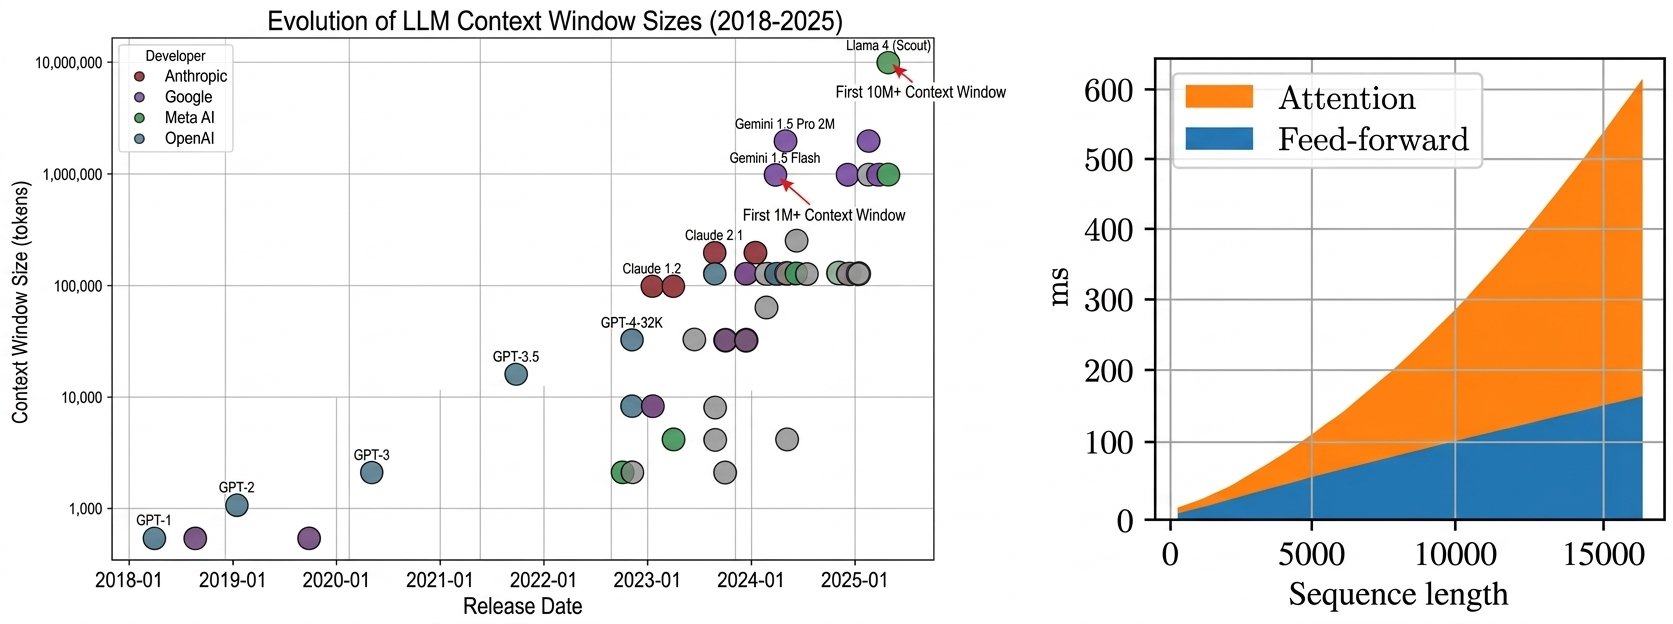
\includegraphics[width=1\linewidth]{context.jpg}
\end{figure}

\begin{itemize}
    \item Combine local \(+\) global attention.
    \item Systems engineering.
\end{itemize}

But what if we want more radical and potentially large gains?

\subsubsection*{Linear attention}

Consider the normal attention operation .. \(Q \in \mathbb{R}^{n \times d_k}\), \(K \in \mathbb{R}^{n \times d_k}\) and \(V \in \mathbb{R}^{n \times d_v}\) ..
\[
    Attn(Q, K, V) = \rho(QK^T)V.
\]

This is quadratic due to \(QK^T\) (\(n^2d_k\)). Can we do better (when \(\rho\) is the identity)?
\[
    (QK^T)V = Q(K^TV).
\]

This is very silly, but surprisingly important .. we get from \(n^2d_k + n^2d_v\) to \(2nd_kd_v\).

\subsubsection*{Recurrent form of linear attention}

This is linear time (great) but the even nicer thing is that this looks like a RNN ...
\[
    S_t = S_{t - 1} + k_tv_t^T \text{ and } y_t = q_t^TS_t.
\]

This "duality" allows us to train efficiently (using the parallel, quadratic form) and inference efficiently (using the serial, linear form). \\

Note: if one weights \(S_{t - 1}\) by \(\gamma\), you get RetNet.

\subsubsection*{Minimax M1}

\begin{figure}[hpbt]
    \centering
    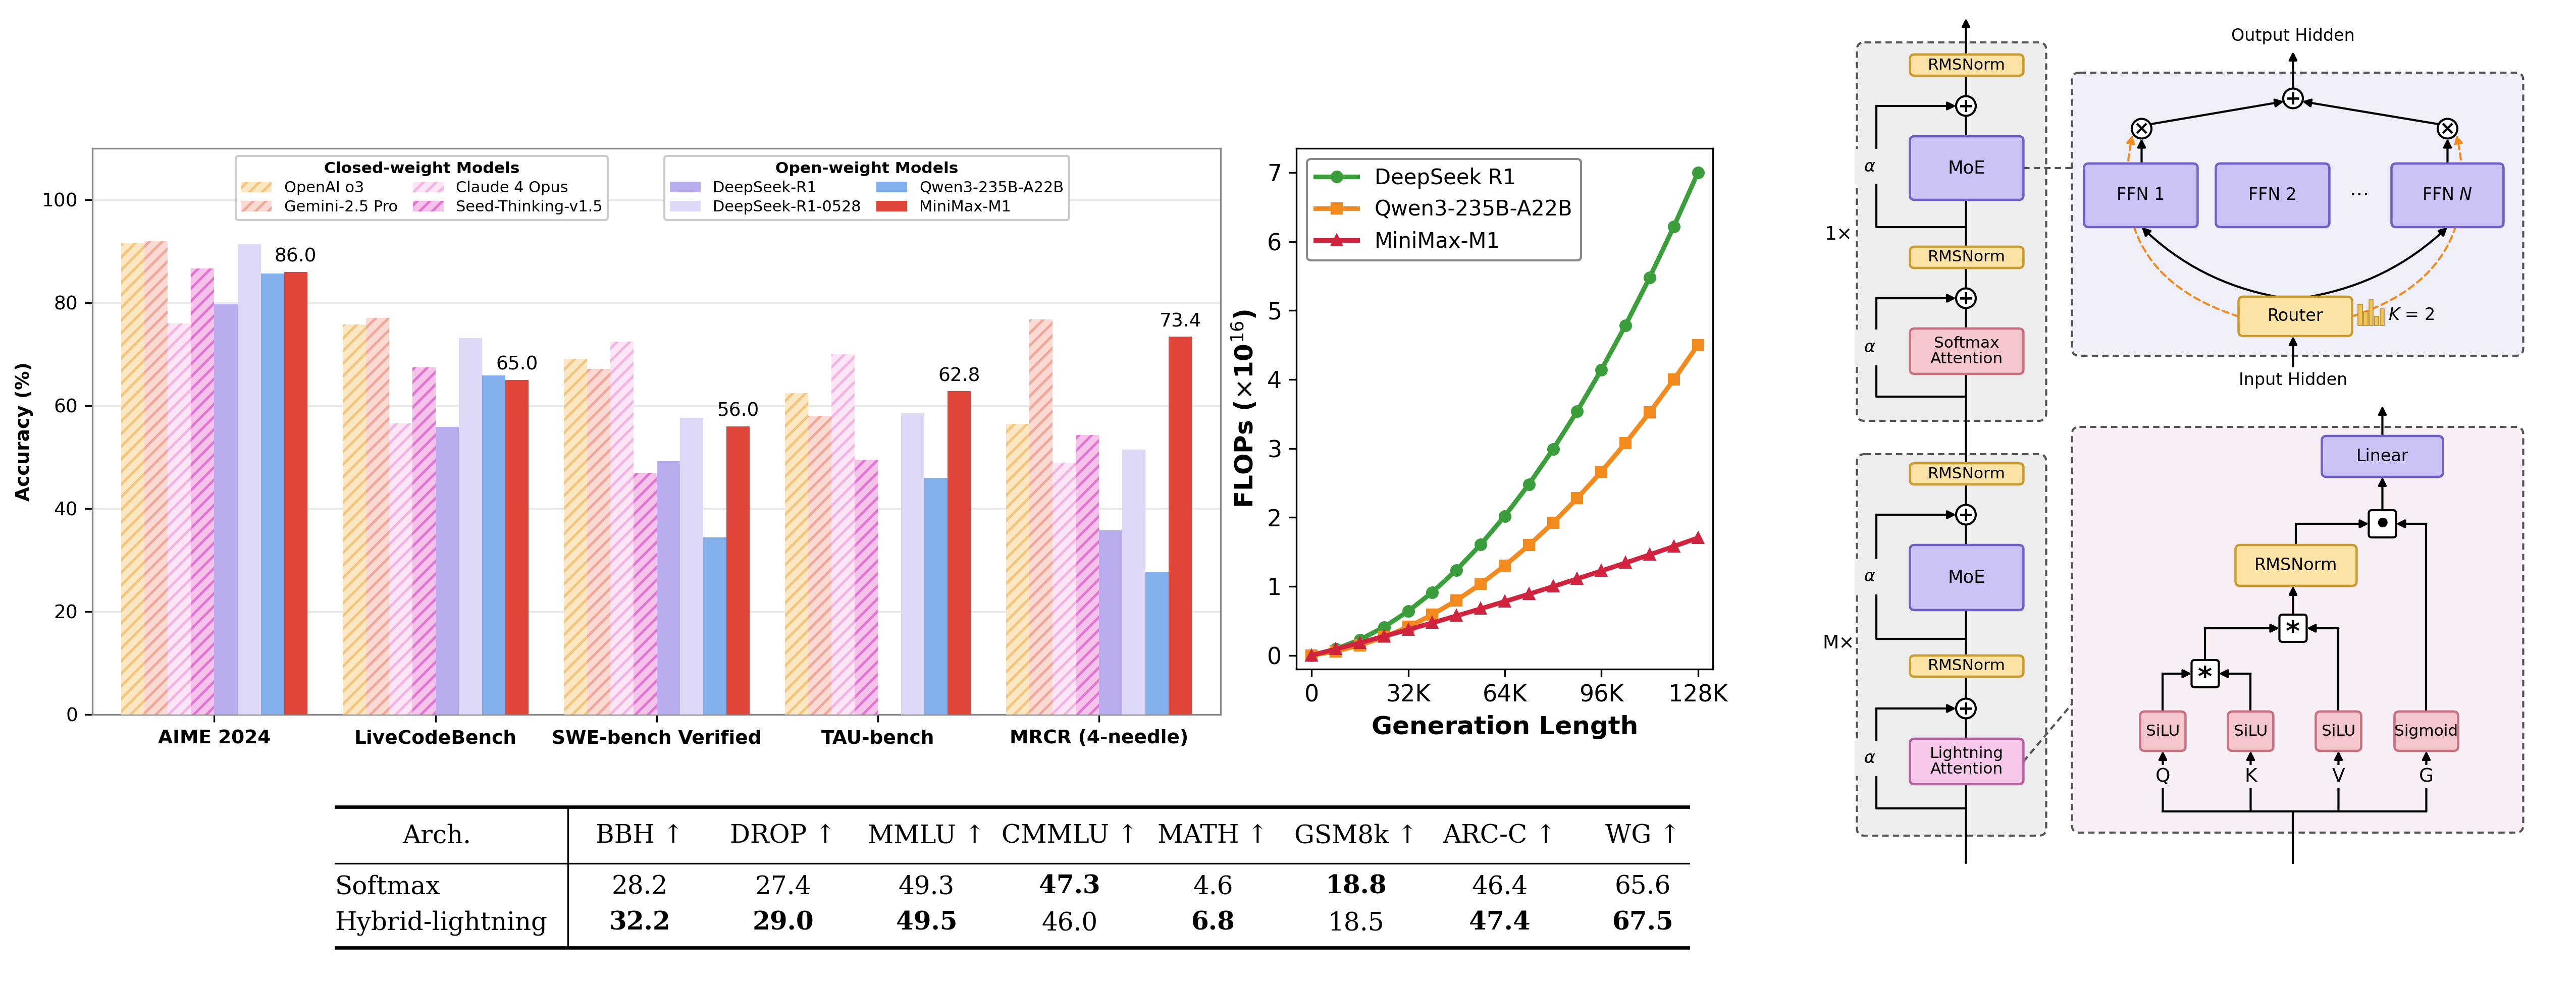
\includegraphics[width=1\linewidth]{minimax.png}
\end{figure}

\begin{remark}
    Minimax M1 (and minimax-text-01) use a 7-to-1 hybrid (7 linear, 1 full) linear attention.
\end{remark}

Performance (generally) seems strong, and they show linear scaling in context length.

\subsubsection*{From linear attention to Mamba-2}

Let's generalize linear attention a liitle bit and add per-position weights .. 
\[
    S_{t} = \gamma_tS_{t - 1} + k_tv_t^T \text{ and } y_t = q_t^TS_t + v_t^TD \text{ with } \gamma_t = f(x_t).
\]

There is a lot more words to justify this (go read the Mamba-2 paper) but the mechanics is that we can make linear attention more expressive via gating (gating is good)!

\begin{remark}
    This continues to have duality properties (compute \(\gamma\) in parallel, apply duality).
\end{remark}

\subsubsection*{Nemotron 3}

Mamba attention hybrid (3-1 ish) - comparable (or better) performance to other similar models.

\subsubsection*{Gated delta net (and friends)}

Let's generalize things further - gate the input and selectively erase state ..
\[
    S_{t} = \gamma_t(I - \beta_tk_tk_t^T)S_{t - 1} + \beta_tk_tv_t^T \text{ and } y_t = q_t^TS_t \text{ with } \gamma_t = f(x_t) \text{ and } \beta_t = f(x_t).
\]

The gated delta net adds a "no input operation" gate (\(\beta = 0\)) and \textit{erases} anything in the direction of the current key (\(I - \beta_tk_tk_t^T\)).

\begin{remark}
    Close relationships to various fast weight programming / test time training ideas.
\end{remark}

\subsubsection*{Qwen 3.5 / Next}

\begin{figure}[hpbt]
    \centering
    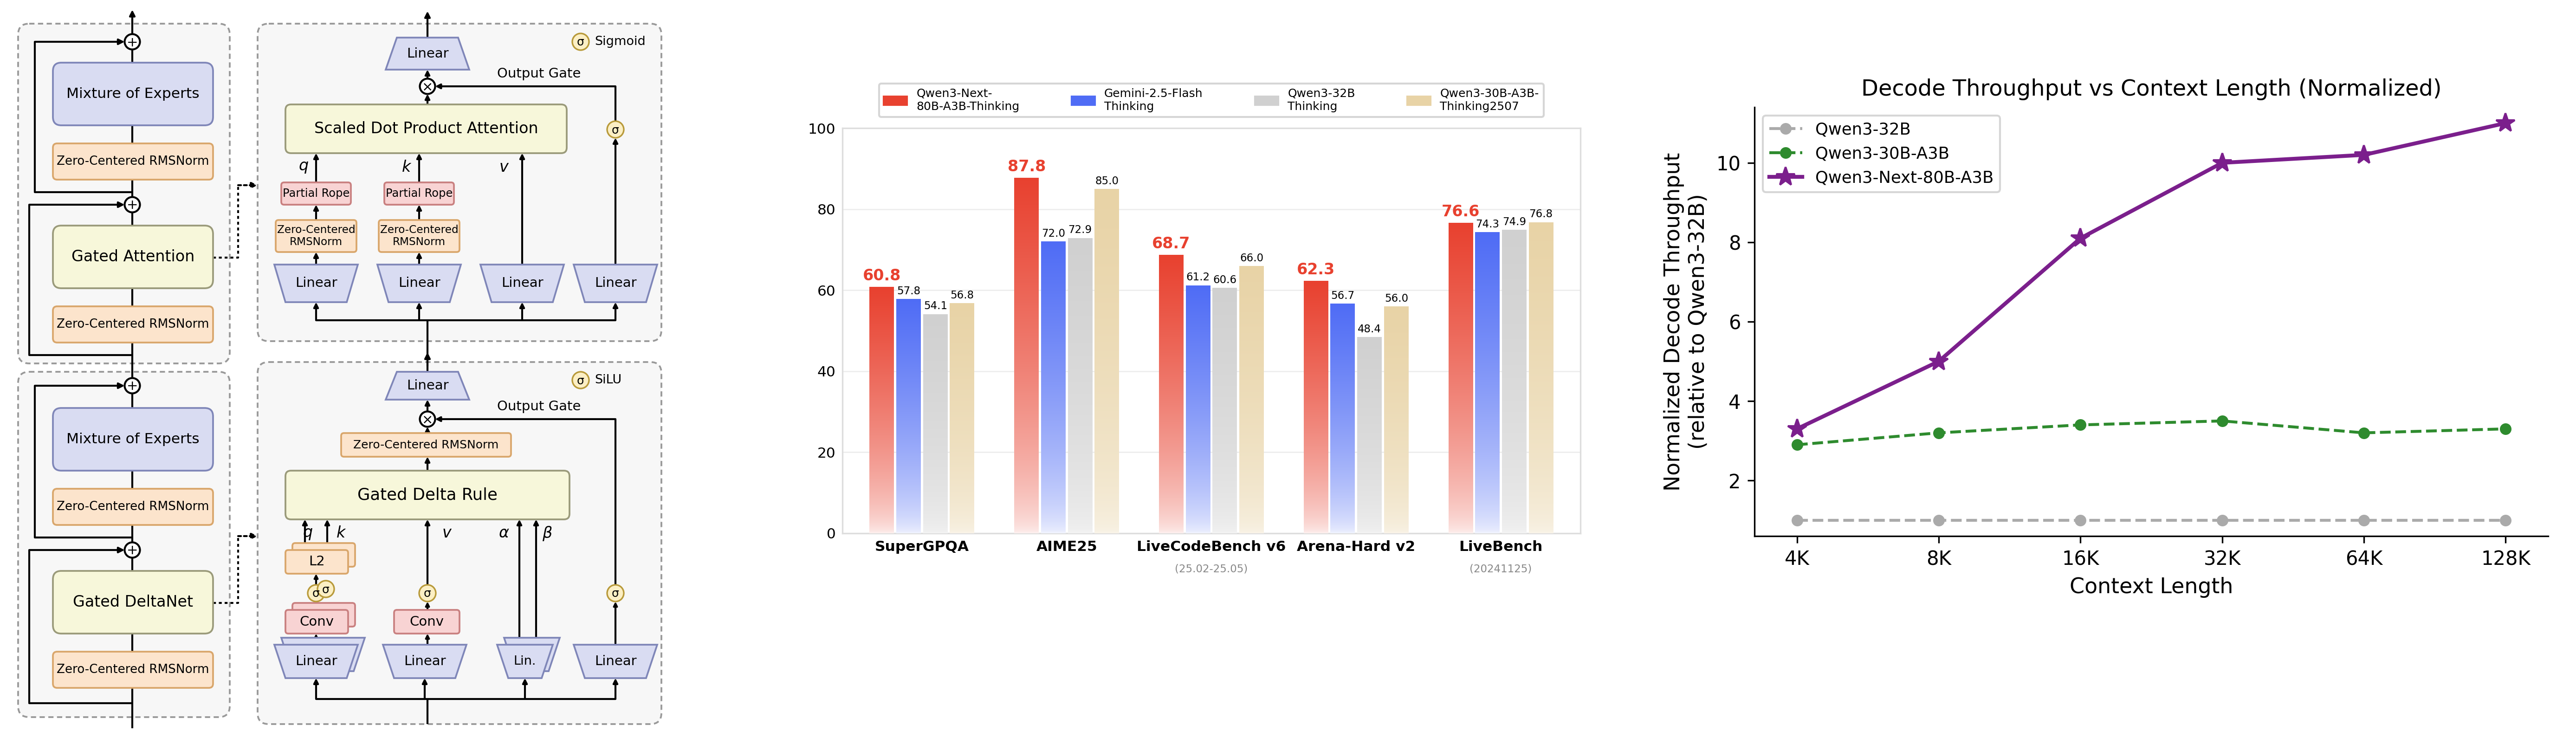
\includegraphics[width=1\linewidth]{qwen.png}
\end{figure}

The newest Qwen are 3-1 GDN / attention hybrids. Once again, pretty reasonable performance with good inference characteristics.

Not many controlled ablations, but some evidence of low losses at small hybrid scales. 

\subsubsection*{Alternative to hybrids: sparse adaption}

Instead of attending to every token, do sparse attention (DSA) \\

\textbf{Prototype of DSA.} The prototype of DSA (DeepSeek Attention) primarily consists of two components: a lightning indexer and a fine-grained token selection mechanism. \\

The \textbf{lightning indexer} computes the index score \(I_{t, s}\) between the query token \(h_t \in \mathbb{R}^d\) and a preceding token \(h_s \in \mathbb{R}^d\), determining which tokens to be selected by the query token: 
\[
    I_{t, s} = \sum_{j = 1}^{H^I}w_{t,j}^I \cdot \text{ReLU}(q_{t, j}^I \cdot k_s^I),
\]
where \(H^I\) denotes the number of indexer heads; \(q_{t,j}^I \in \mathbb{R}^{d^I}\) and \(w_{t, j}^I \in \mathbb{R}\) are derived from the query token \(h_t\) and \(k_s^I \in \mathbb{R}^{d^I}\) is derived from the preceding token \(h_s\)

\begin{remark}
    We choose the ReLU as the activation function for throughput considerations. Given the lightning indexer has a small number of heads and can be implemented in FP8, its computational efficiency is remarkable.
\end{remark}

Given the indexer scores \(\{I_{t, s}\}\) for each query token \(h_t\), the \textbf{token selection mechanism} retrieves only the key-value entries \(\{c_s\}\) corresponding to the top-\(k\) index scores. Then, the attention output \(u_t\) is computed by applying the attention mechanism between the query token \(h_t\) and the sparsely selected key-value entries \(\{c_s\}\):
\[
    u_t = \text{Attn}(h_t, \{c_s \mid I_{t, s} \in \text{Top-k}(I_t)\}).
\]

\begin{remark}
    The indexer can be very lightweight, giving significant gains and can be "post-hoc" adapted after dense short context pretraining.
\end{remark}

\subsection*{Mixture of Experts}

\begin{figure}[hpbt]
    \centering
    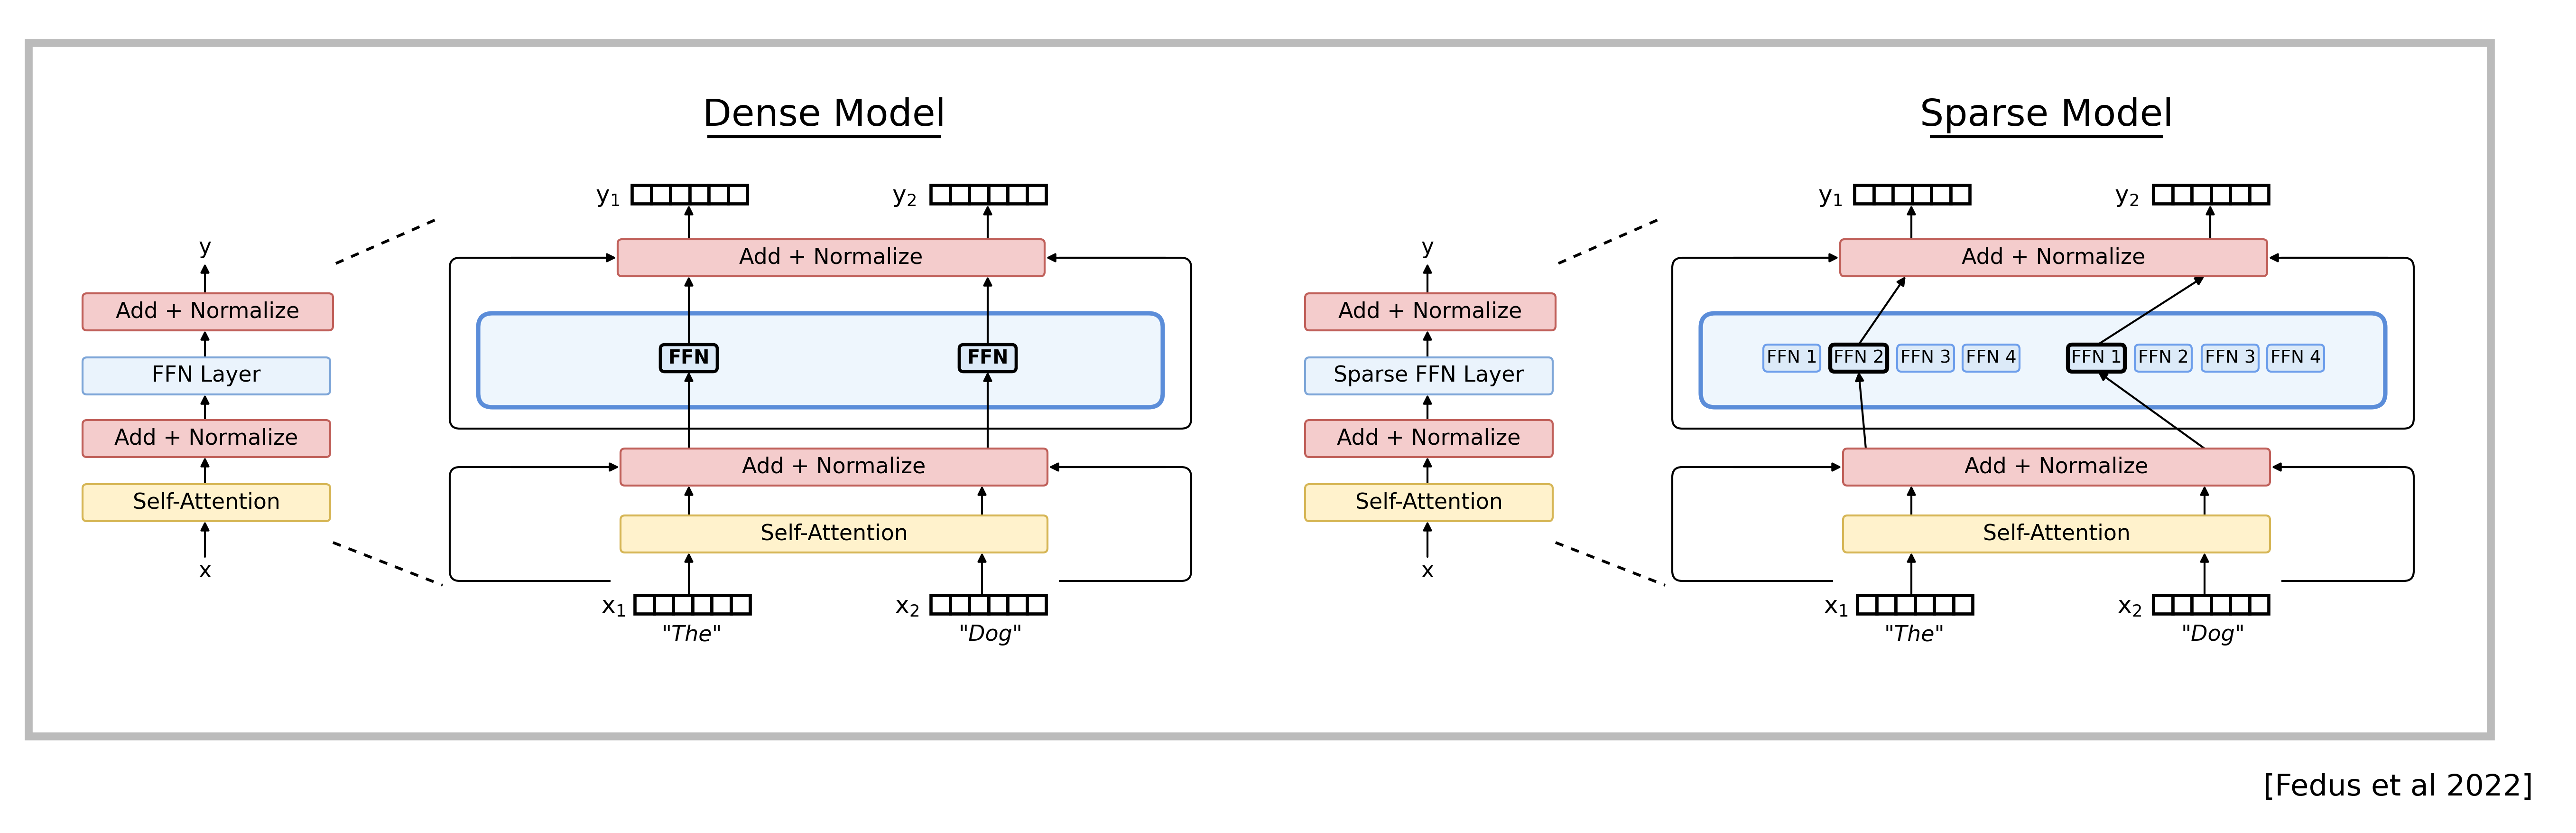
\includegraphics[width=1\linewidth]{sparse.png}
\end{figure}

\subsubsection*{What's a MoE?}

Replace big feedforward with (many) big feedforward networks and a selector layer.

\begin{figure}[hpbt]
    \centering
    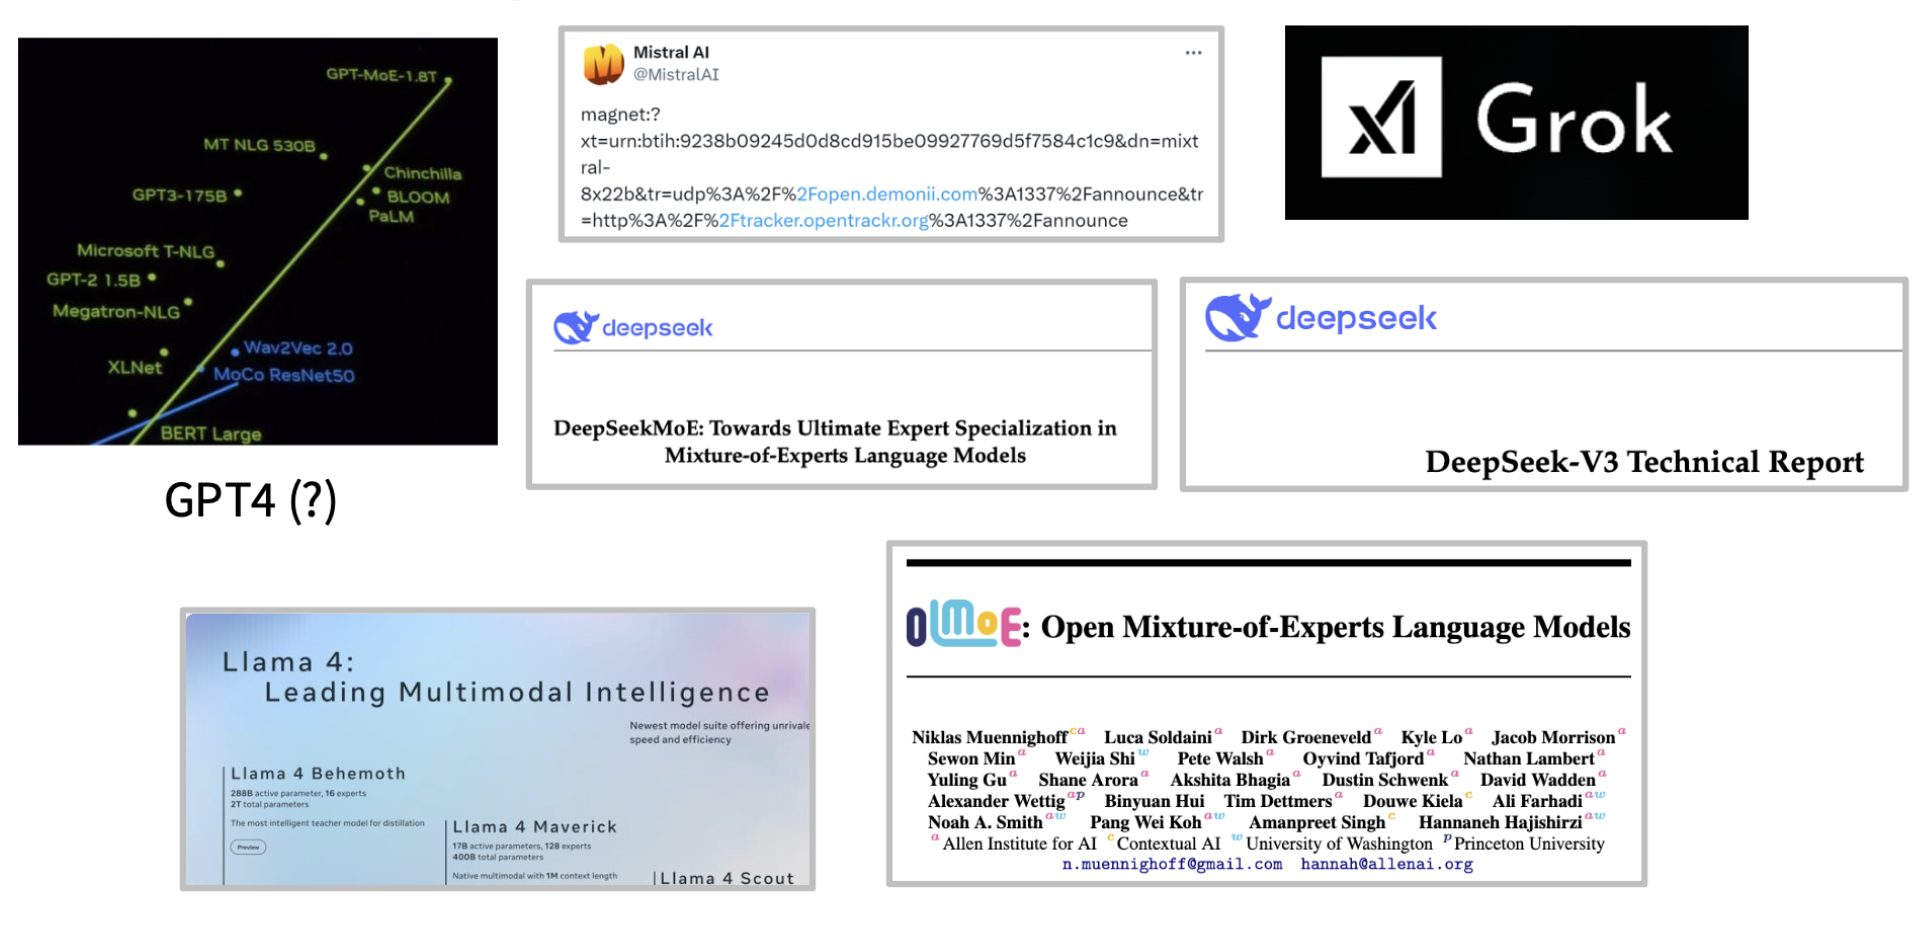
\includegraphics[width=0.62\linewidth]{MoEss.png}
\end{figure}

\begin{claim}
    You can increase the \# experts without affecting FLOPs.
\end{claim}

\subsubsection*{Why are MoEs getting popular?}

\begin{itemize}
    \item Same FLOPs, more parameters does better.
    \item Faster to train MoEs.
    \item \textbf{Highly competitive vs dense equivalents}
    \item Parallelizable to many devices.
\end{itemize}

\begin{figure}[hpbt]
    \centering
    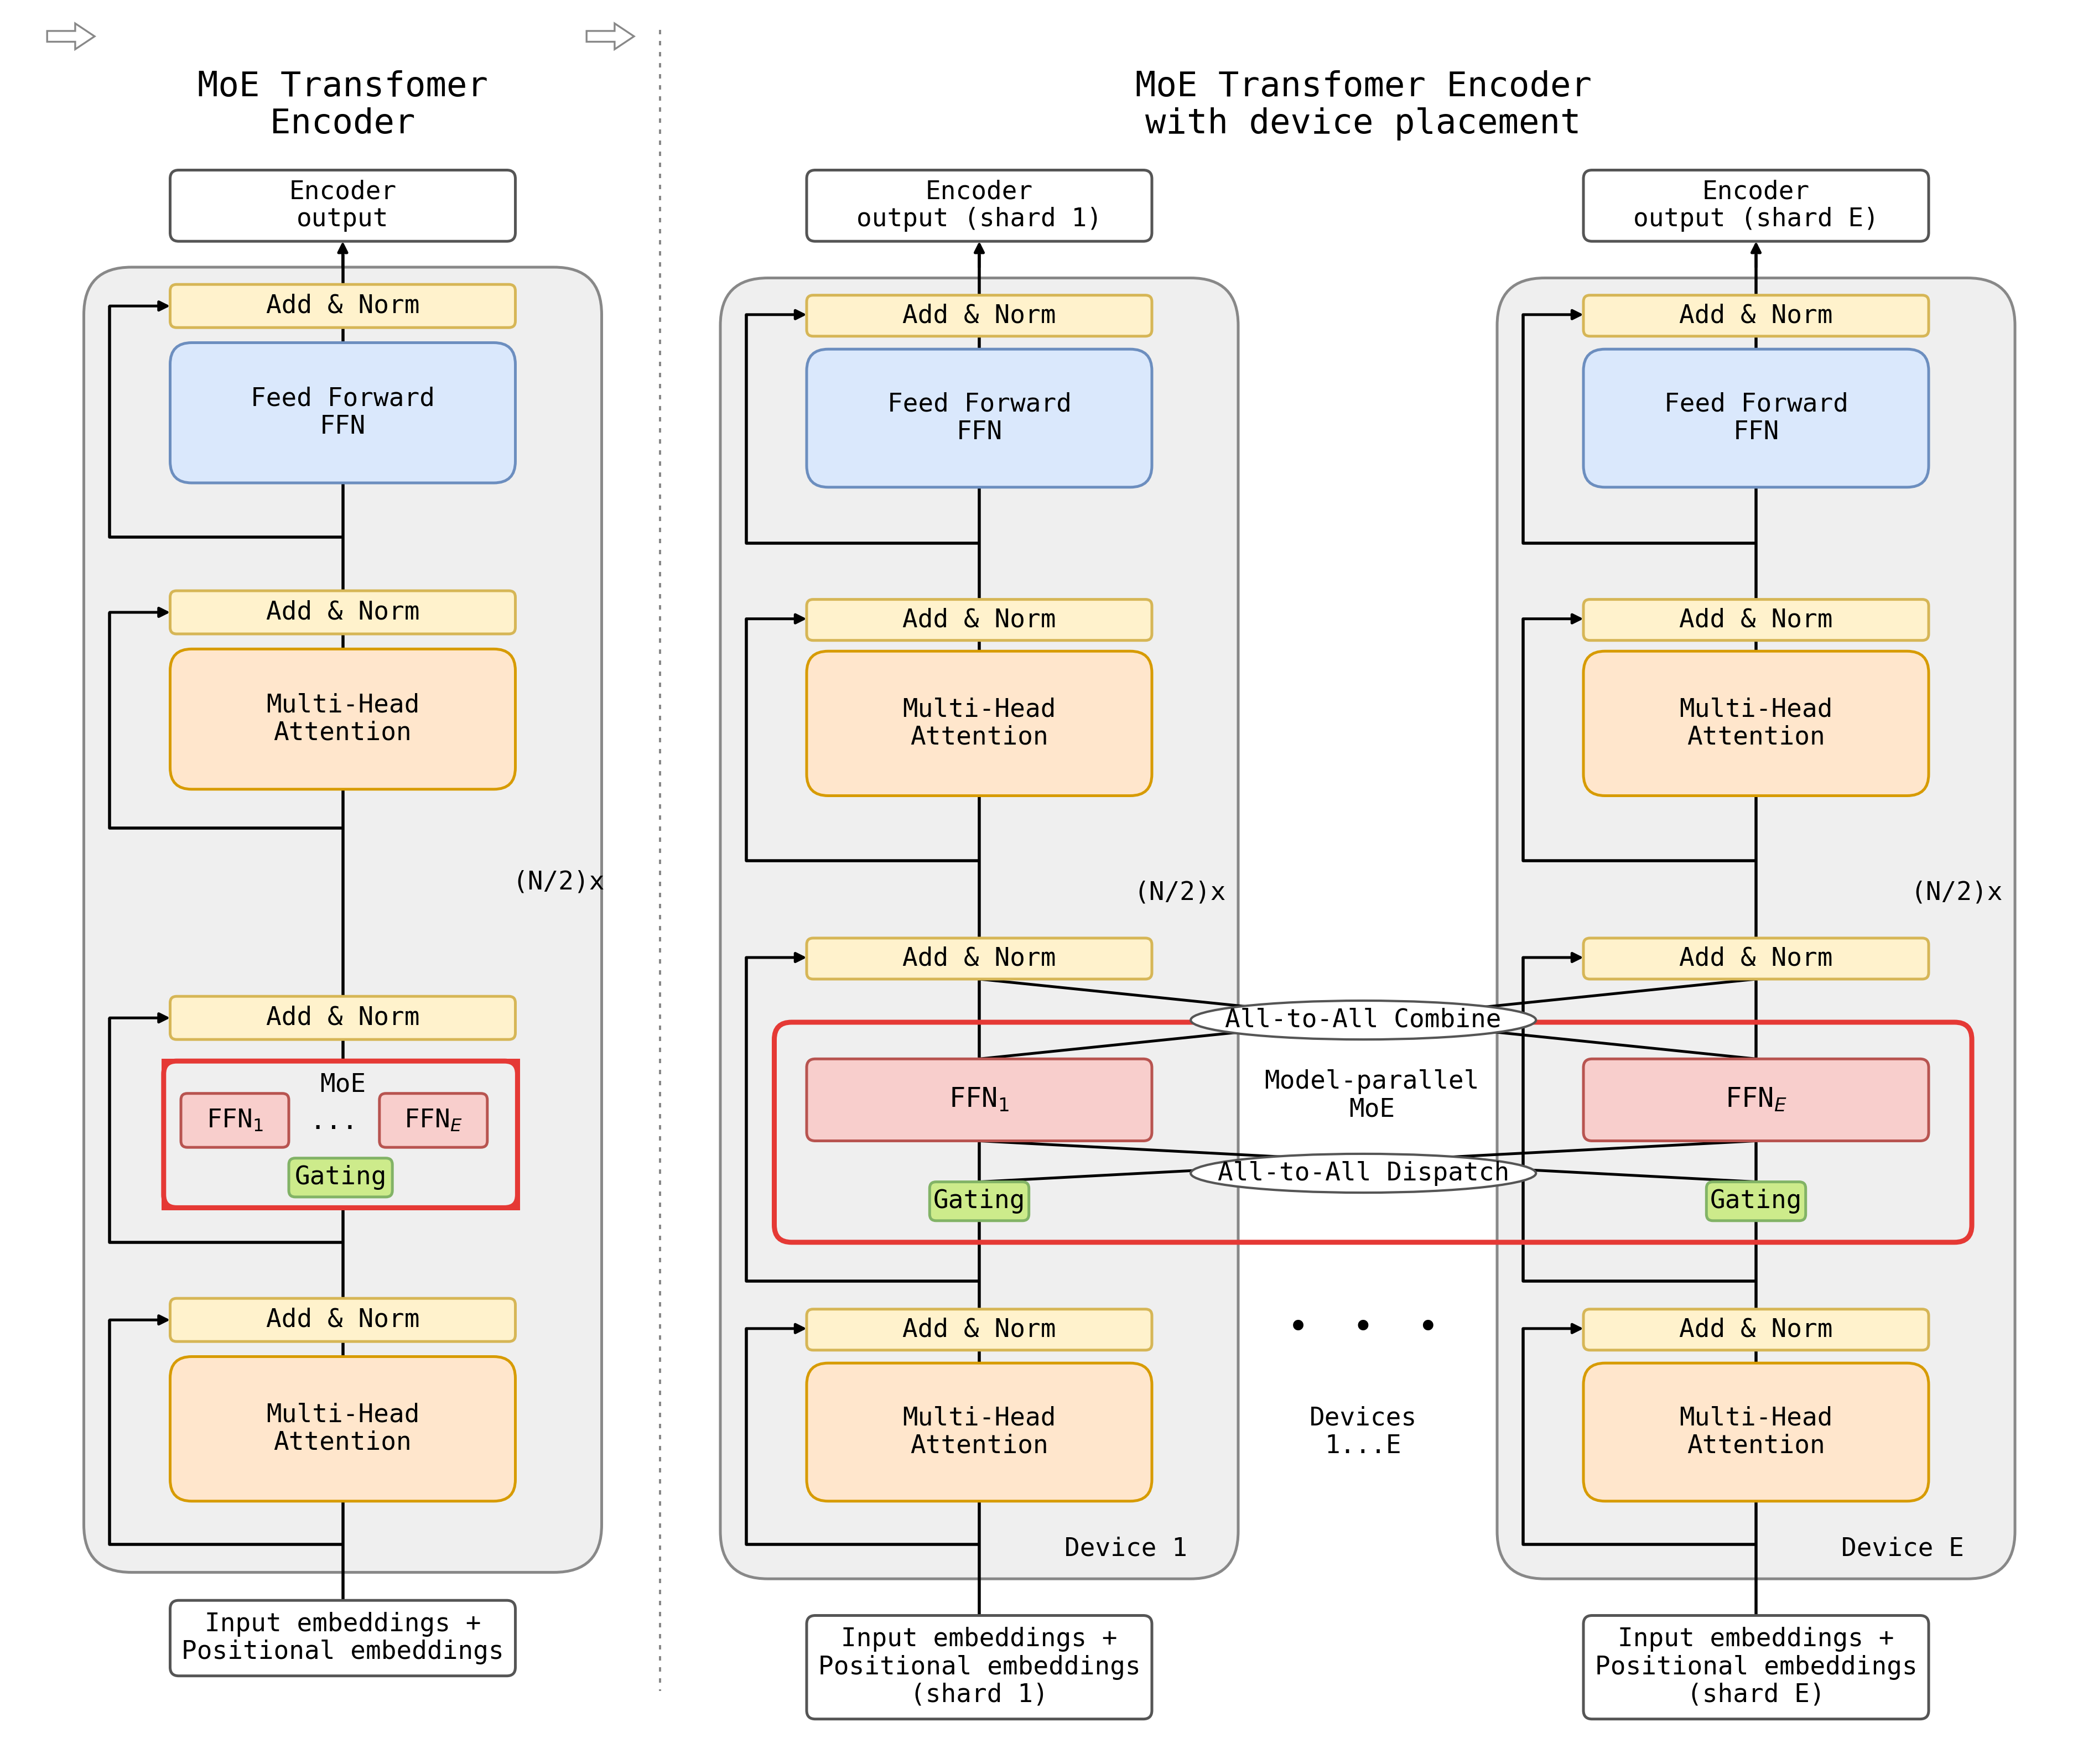
\includegraphics[width=1\linewidth]{systems.png}
\end{figure}

\subsubsection*{Some MoE results - from the West}

\begin{itemize}
    \item MoEs are most of the highest-performance open models and are quite quick.
    \item \textbf{Examples:} LLaMA 4 Maverick, Gemini 2.0 Flash, GPT-4o.
\end{itemize}

\subsubsection*{Earlier MoE results from Chinese groups - Qwen}

Chinese LLM companies are also doing quite a bit of MoE work on the smaller end.

\begin{figure}[hpbt]
    \centering
    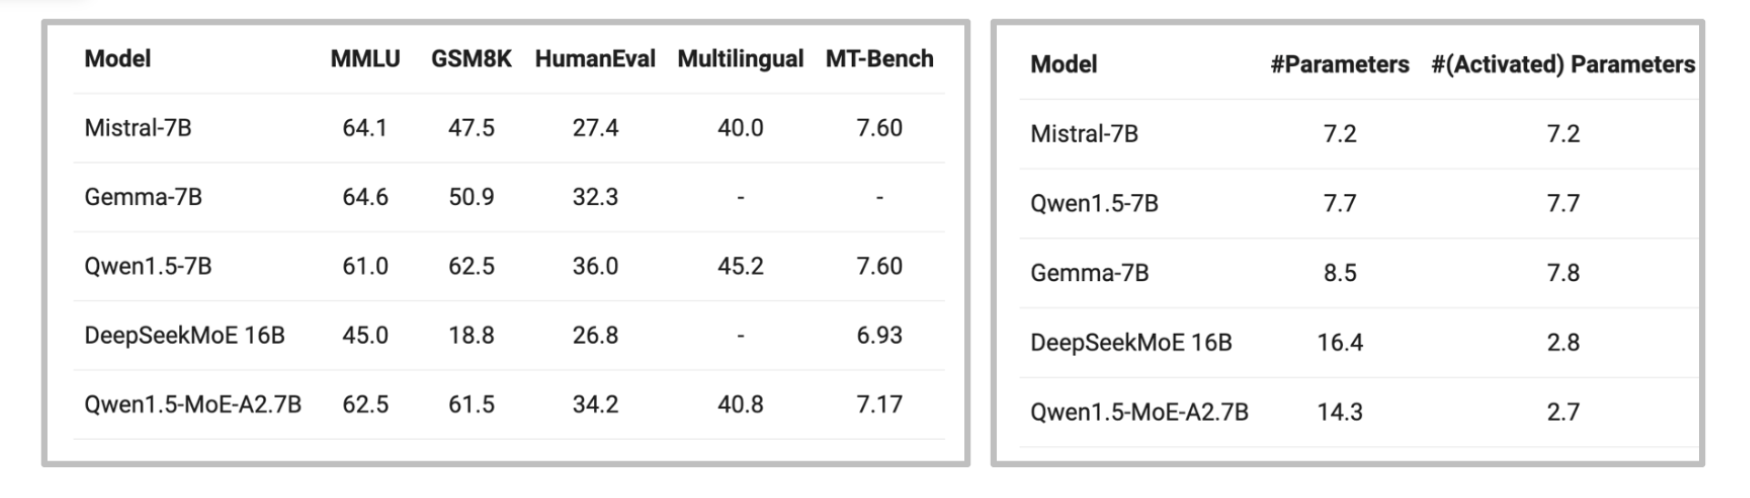
\includegraphics[width=1\linewidth]{chinese.png}
\end{figure}

\subsubsection*{Earlier MoE results from Chinese groups - DeekSeep}

There's also some good ablation work on MoEs showing they're generally good.

\begin{figure}[hpbt]
    \centering
    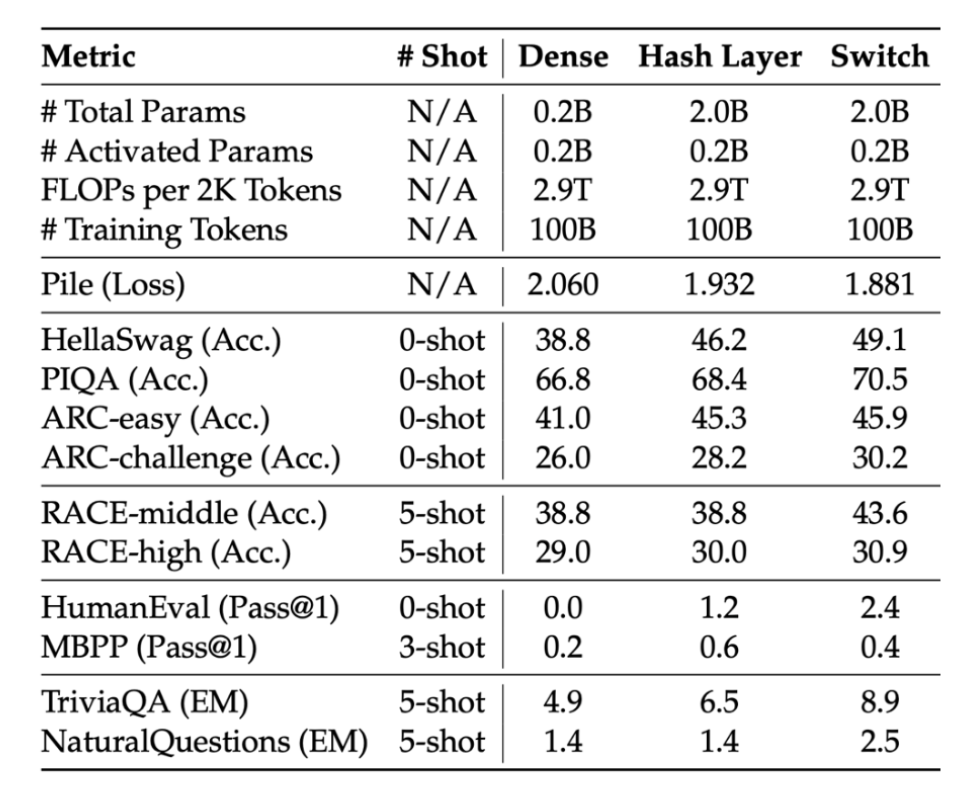
\includegraphics[width=0.8\linewidth]{deepseek.png}
\end{figure}

\subsubsection*{Why haven't MoEs been more popular?}

Infrastructure is complex / advantages on multi-node. 

\begin{center}
    At a high level, sparsity is good when you have accelerators (e.g GPU/TPU) to host all additional parameters that comes when using sparsity. Typically models are trained using data-parallelism where different machines will get different slices of the training/inference data. The machines used for operating on the different slices of the data can now be used to host many more model parameters. Therefore, sparse models are good when training with data-parallelism and/or have high throughput while serving: training/serving on many machines, which can host all of the parameters. [Fedus et al 2022]
\end{center}

Training objectives are somewhat heuristic (and somewhat unstable). 

\subsubsection*{What MoEs generally look like?}

\begin{itemize}
    \item Typical: replace the MLP with MoE layer.
    \item Less common: MoEs for attention heads.
\end{itemize}

\subsubsection*{Routing function - overview}

Many of the routing algorithms boils down to "choose top k". 

\begin{figure}[hpbt]
    \centering
    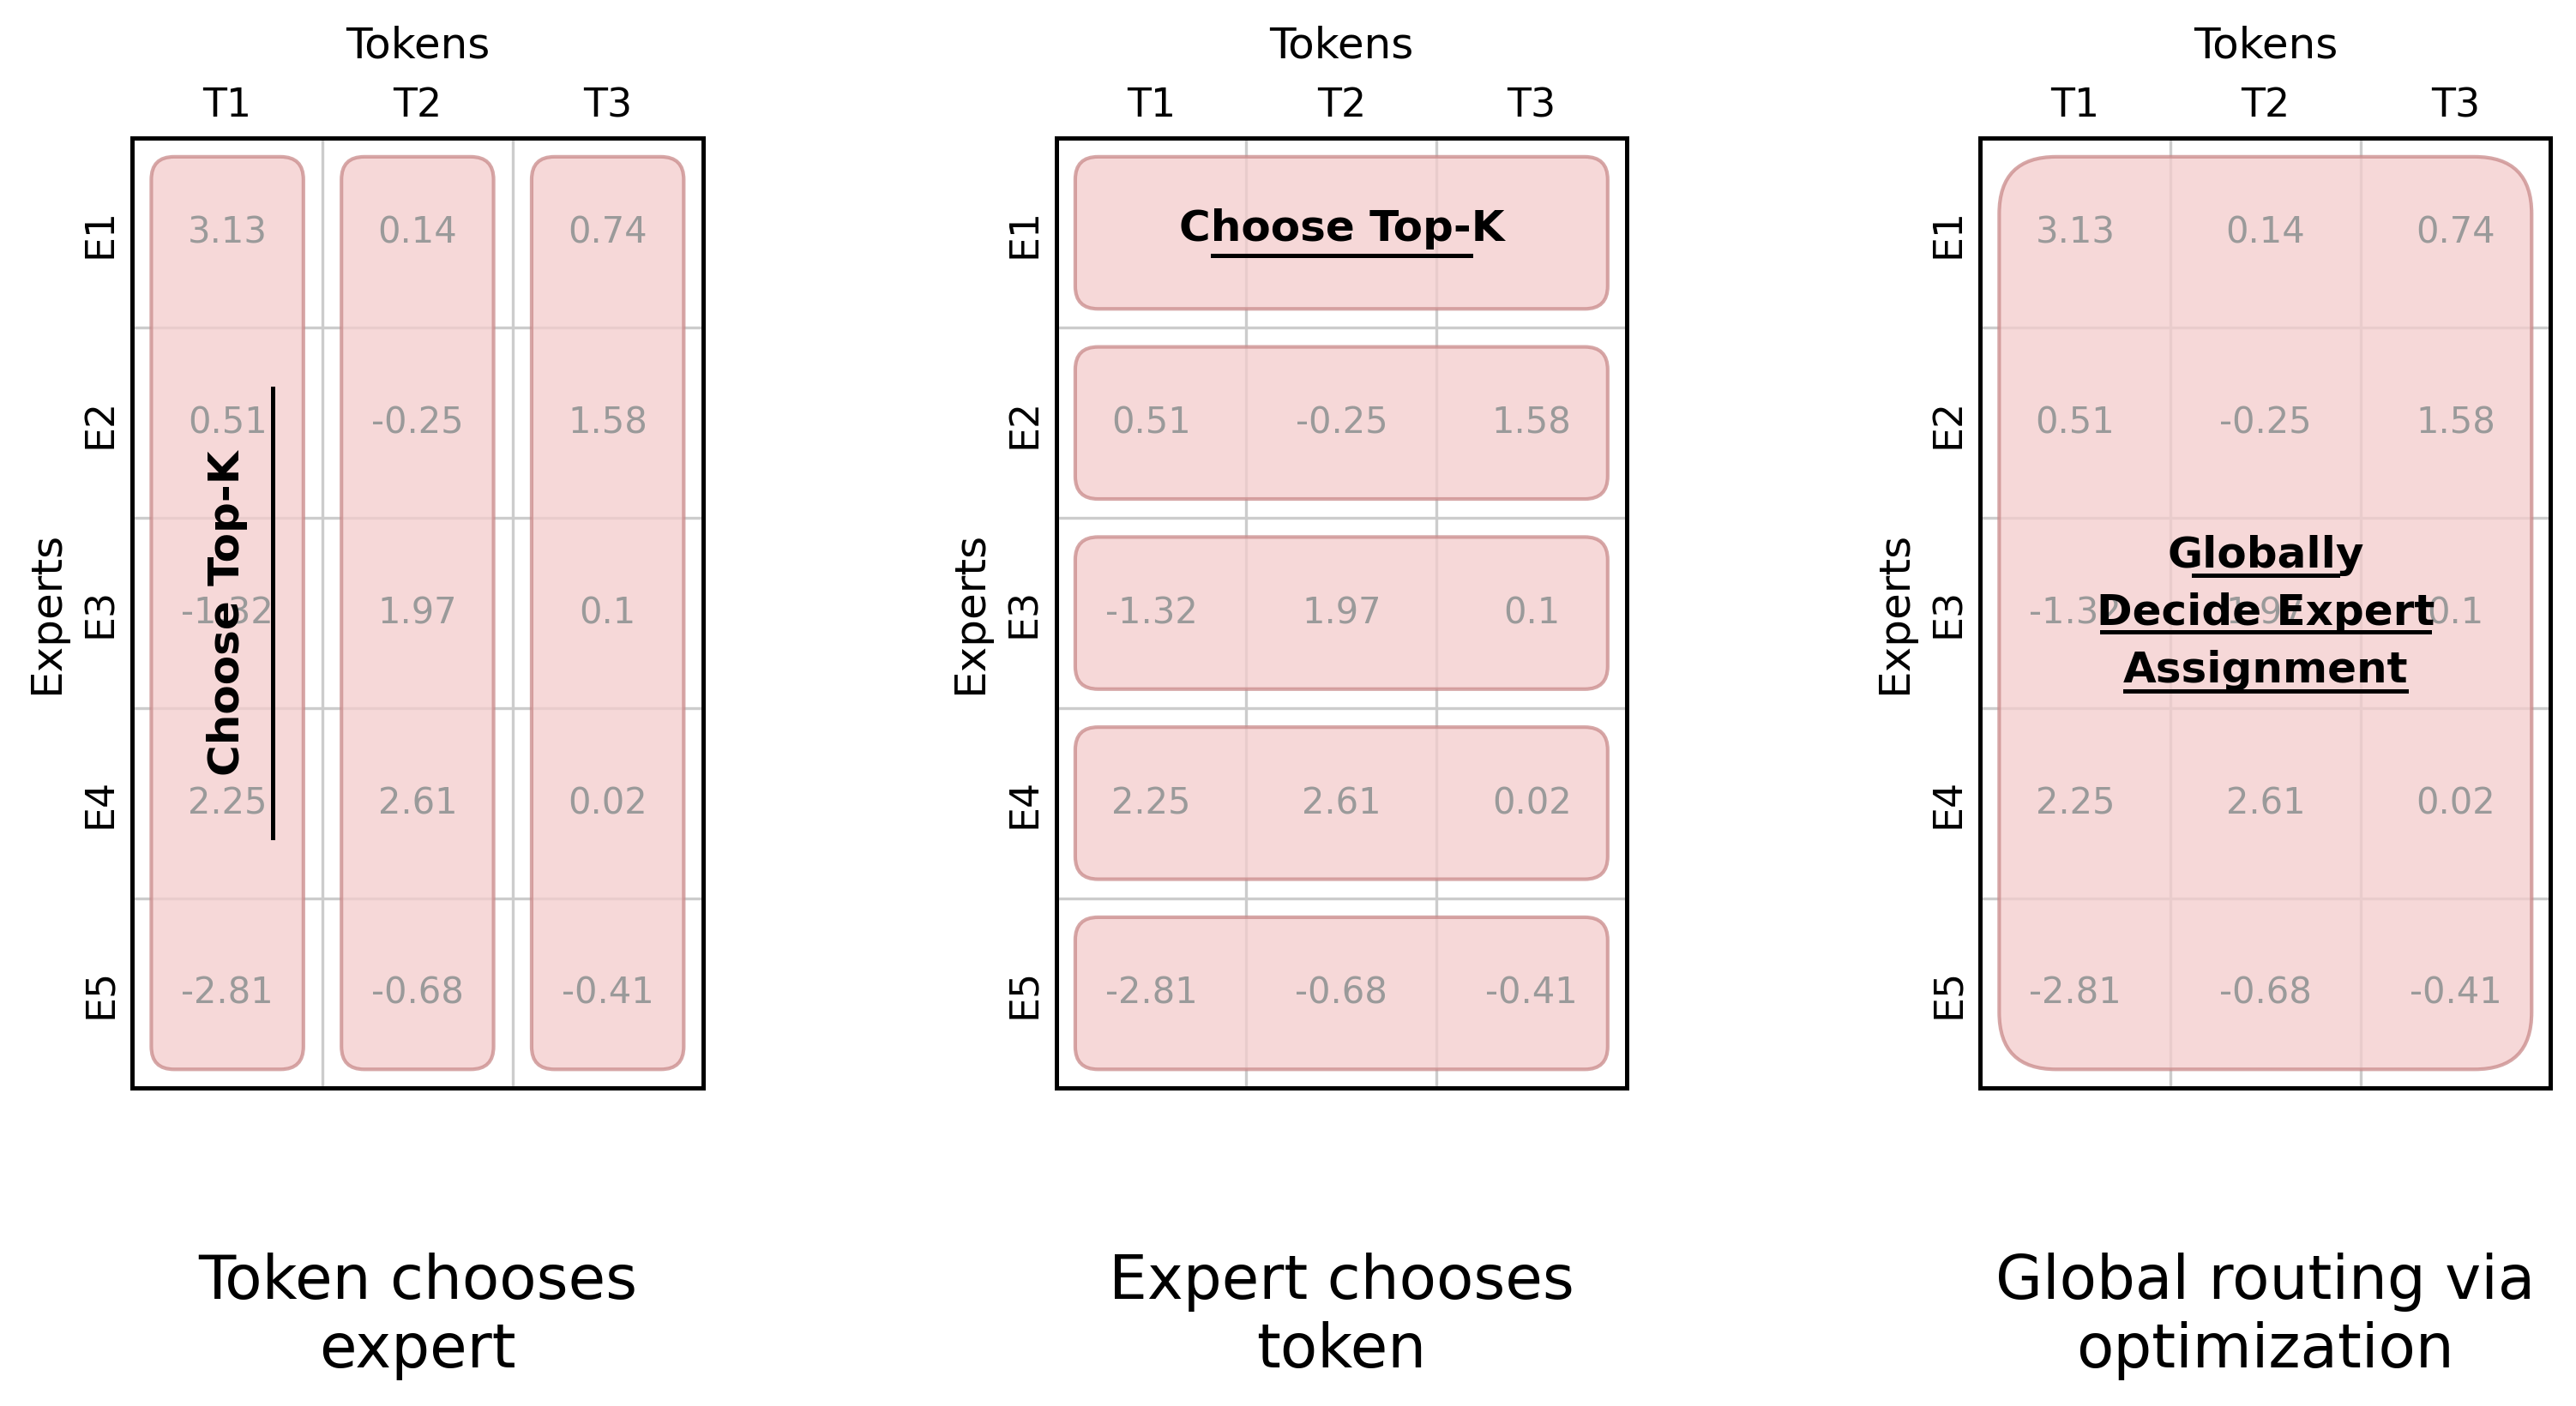
\includegraphics[width=1\linewidth]{routing.png}
\end{figure}

\subsubsection*{Common routing methods}

Almost all the MoEs do a standard "token choice top-\(k\)" routing. 
\begin{itemize}
    \item Top-\(k\): Used in \textit{most} MoEs.
    \item \textbf{Examples:} Switch transformer (\(k = 1\)), Gshard (\(k = 2\)), Grok (\(k = 2\)), Mixtral (\(k = 2\)), Qwen (\(k = 4\)), DBRX (\(k = 4\)), DeepSeek (\(k = 7\)).
    \item Hashing: Used to baseline MoEs.
\end{itemize}

\subsubsection*{Other routing methods}

RL to learn routes.
\begin{itemize}
    \item Used in some of the earliest work
    \item Bengio 2013, not common now
\end{itemize}

Solve a matching problem
\begin{itemize}
    \item Linear assignment for routing
    \item Used in various papers like Clark 2022
\end{itemize}

\subsubsection*{Top-k routing in detail}

Most papers do the old and classic top-k routing. How does it work?

\begin{itemize}
    \item This is the DeepSeek (v1-2) router (Grok, Qwen do this too).
    \begin{figure}[hpbt]
        \centering
        \includegraphics[width=0.6\linewidth]{equations.png}
    \end{figure}
    \item Mistral, DBRX, DeepSeek v3 softmaxes after the TopK. 
\end{itemize}

\subsubsection*{Recent variations from DeepSeek and other Chinese LMs}

\begin{figure}[H]
    \centering
    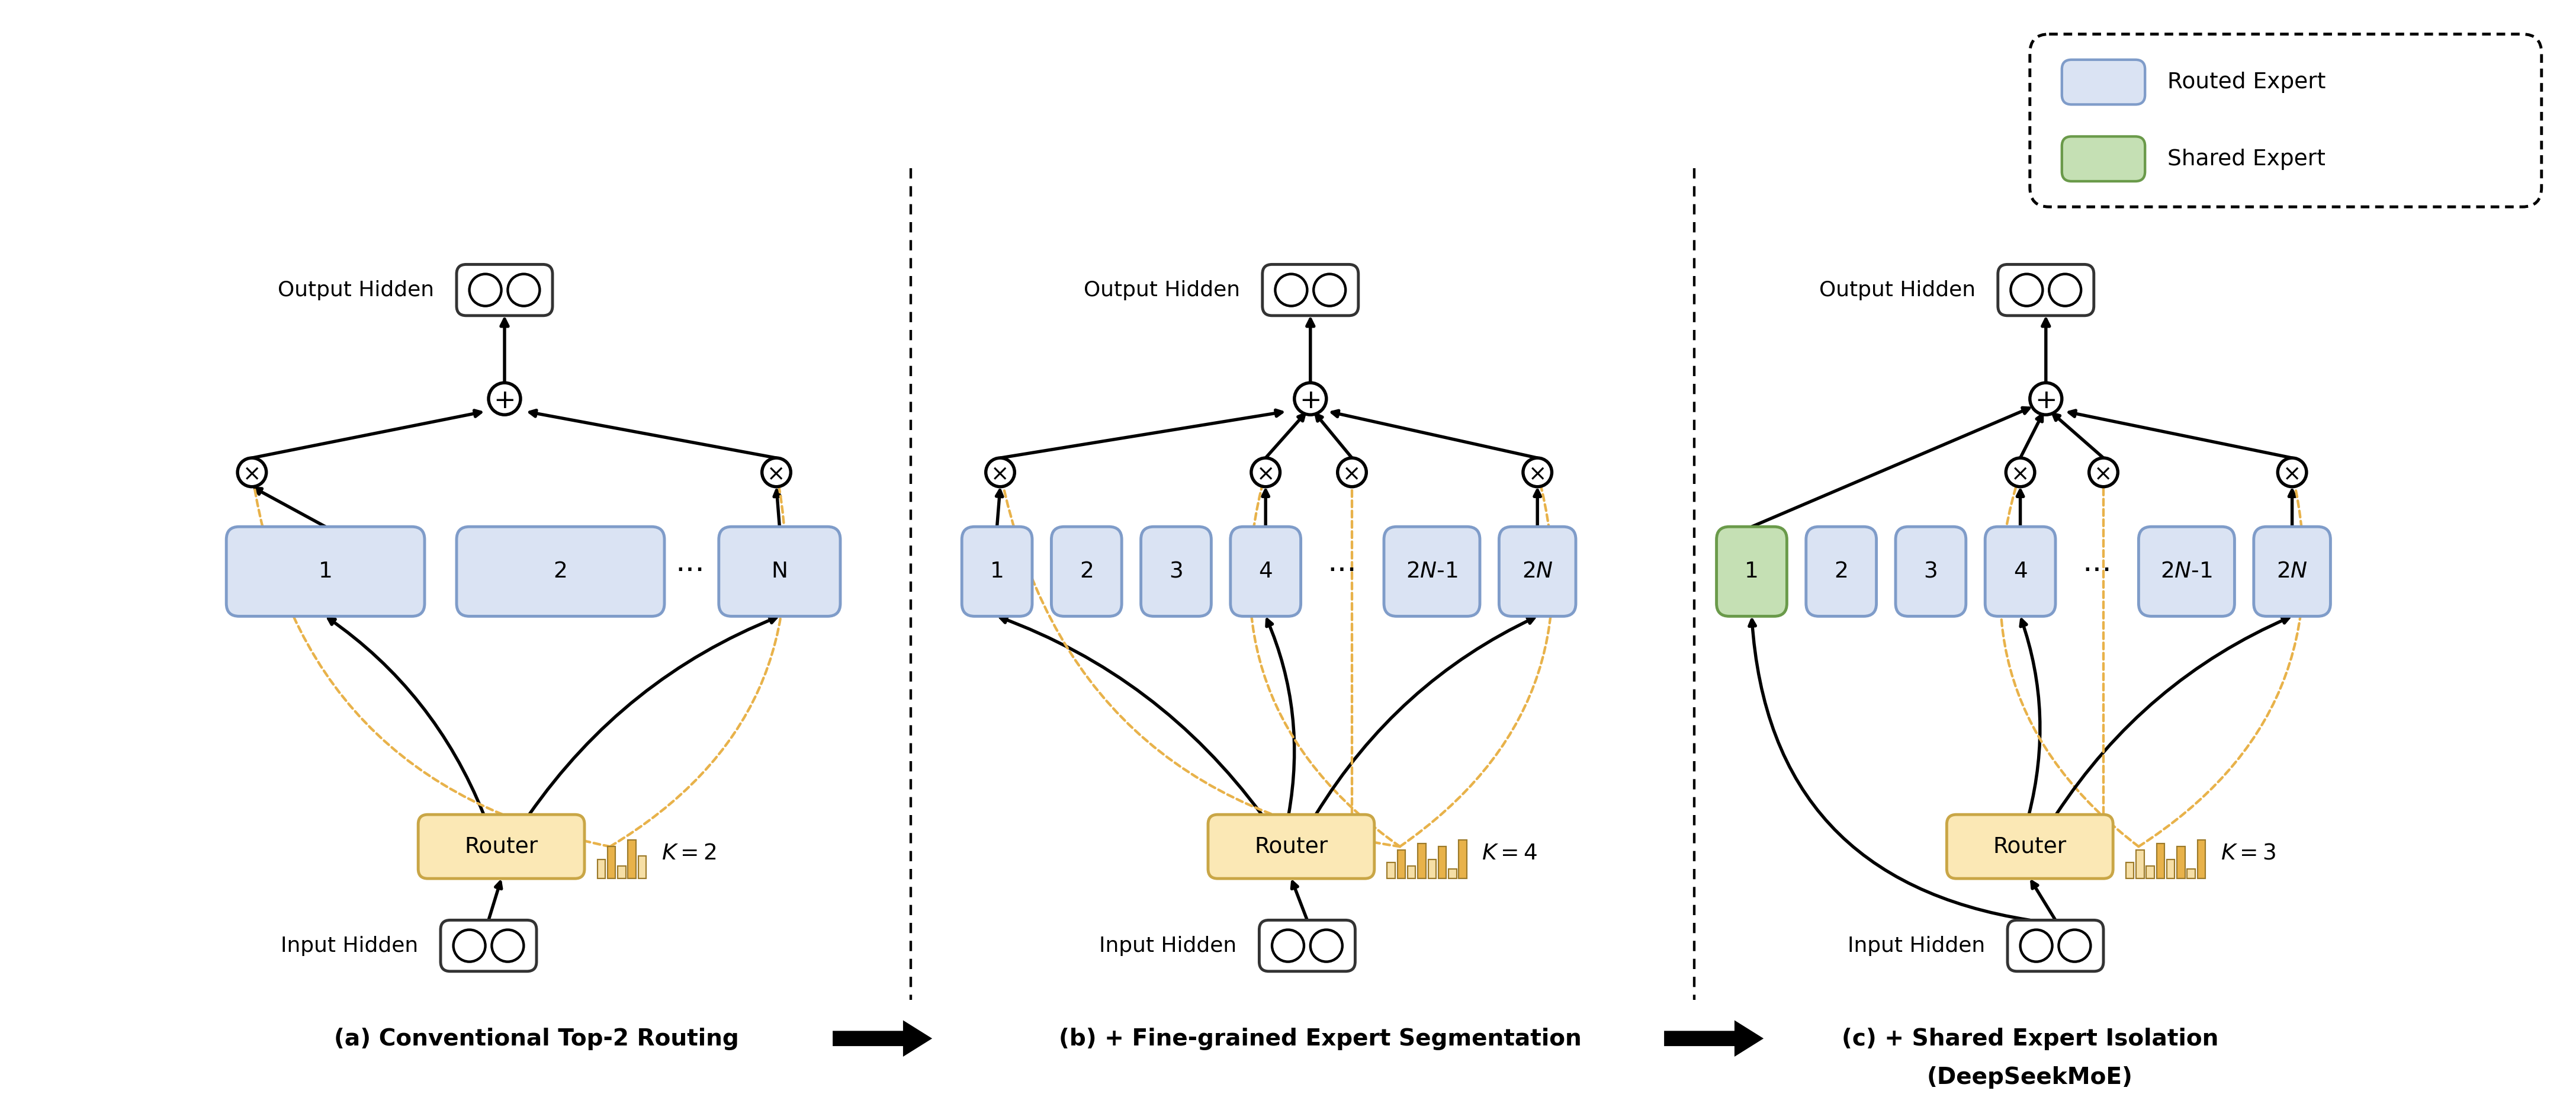
\includegraphics[width=1\linewidth]{shared.png}
\end{figure}

Smaller, larger number of experts \(+\) a few shared experts that are always on.

\subsubsection*{Various ablations from the DeepSeek paper}

\begin{figure}[hpbt]
    \centering
    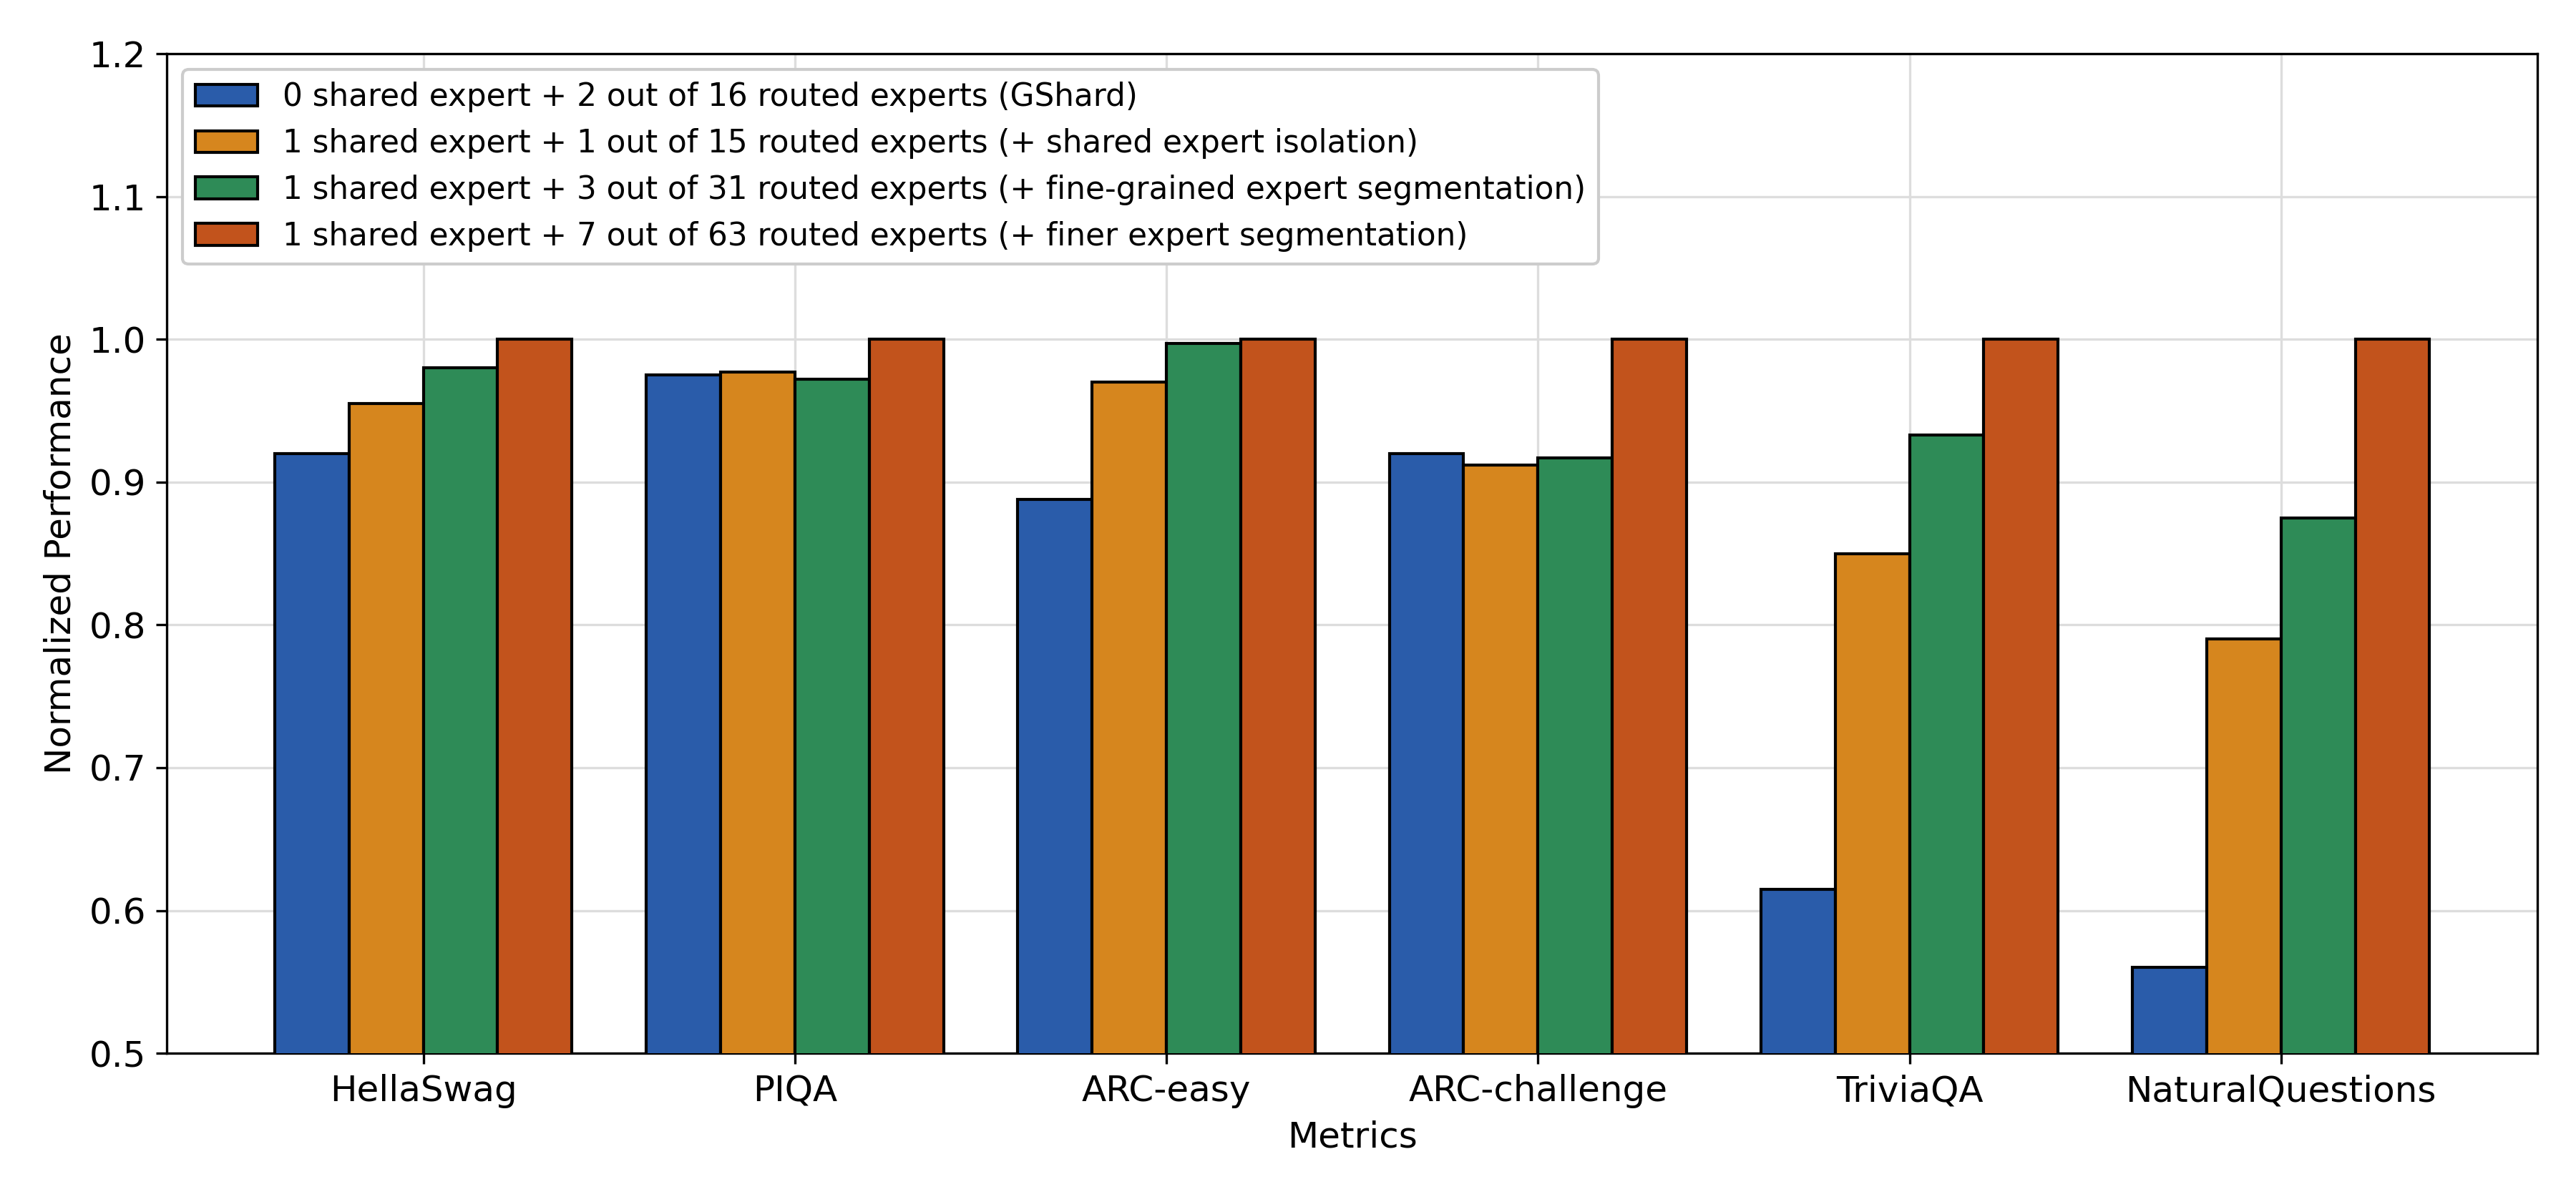
\includegraphics[width=1\linewidth]{evidence.png}
\end{figure}

More experts, shared experts all seem to generally help.

\subsubsection*{Ablations from OlMoE}

Gains from fine-grained experts, none from shared experts.

\begin{figure}[H]
    \centering
    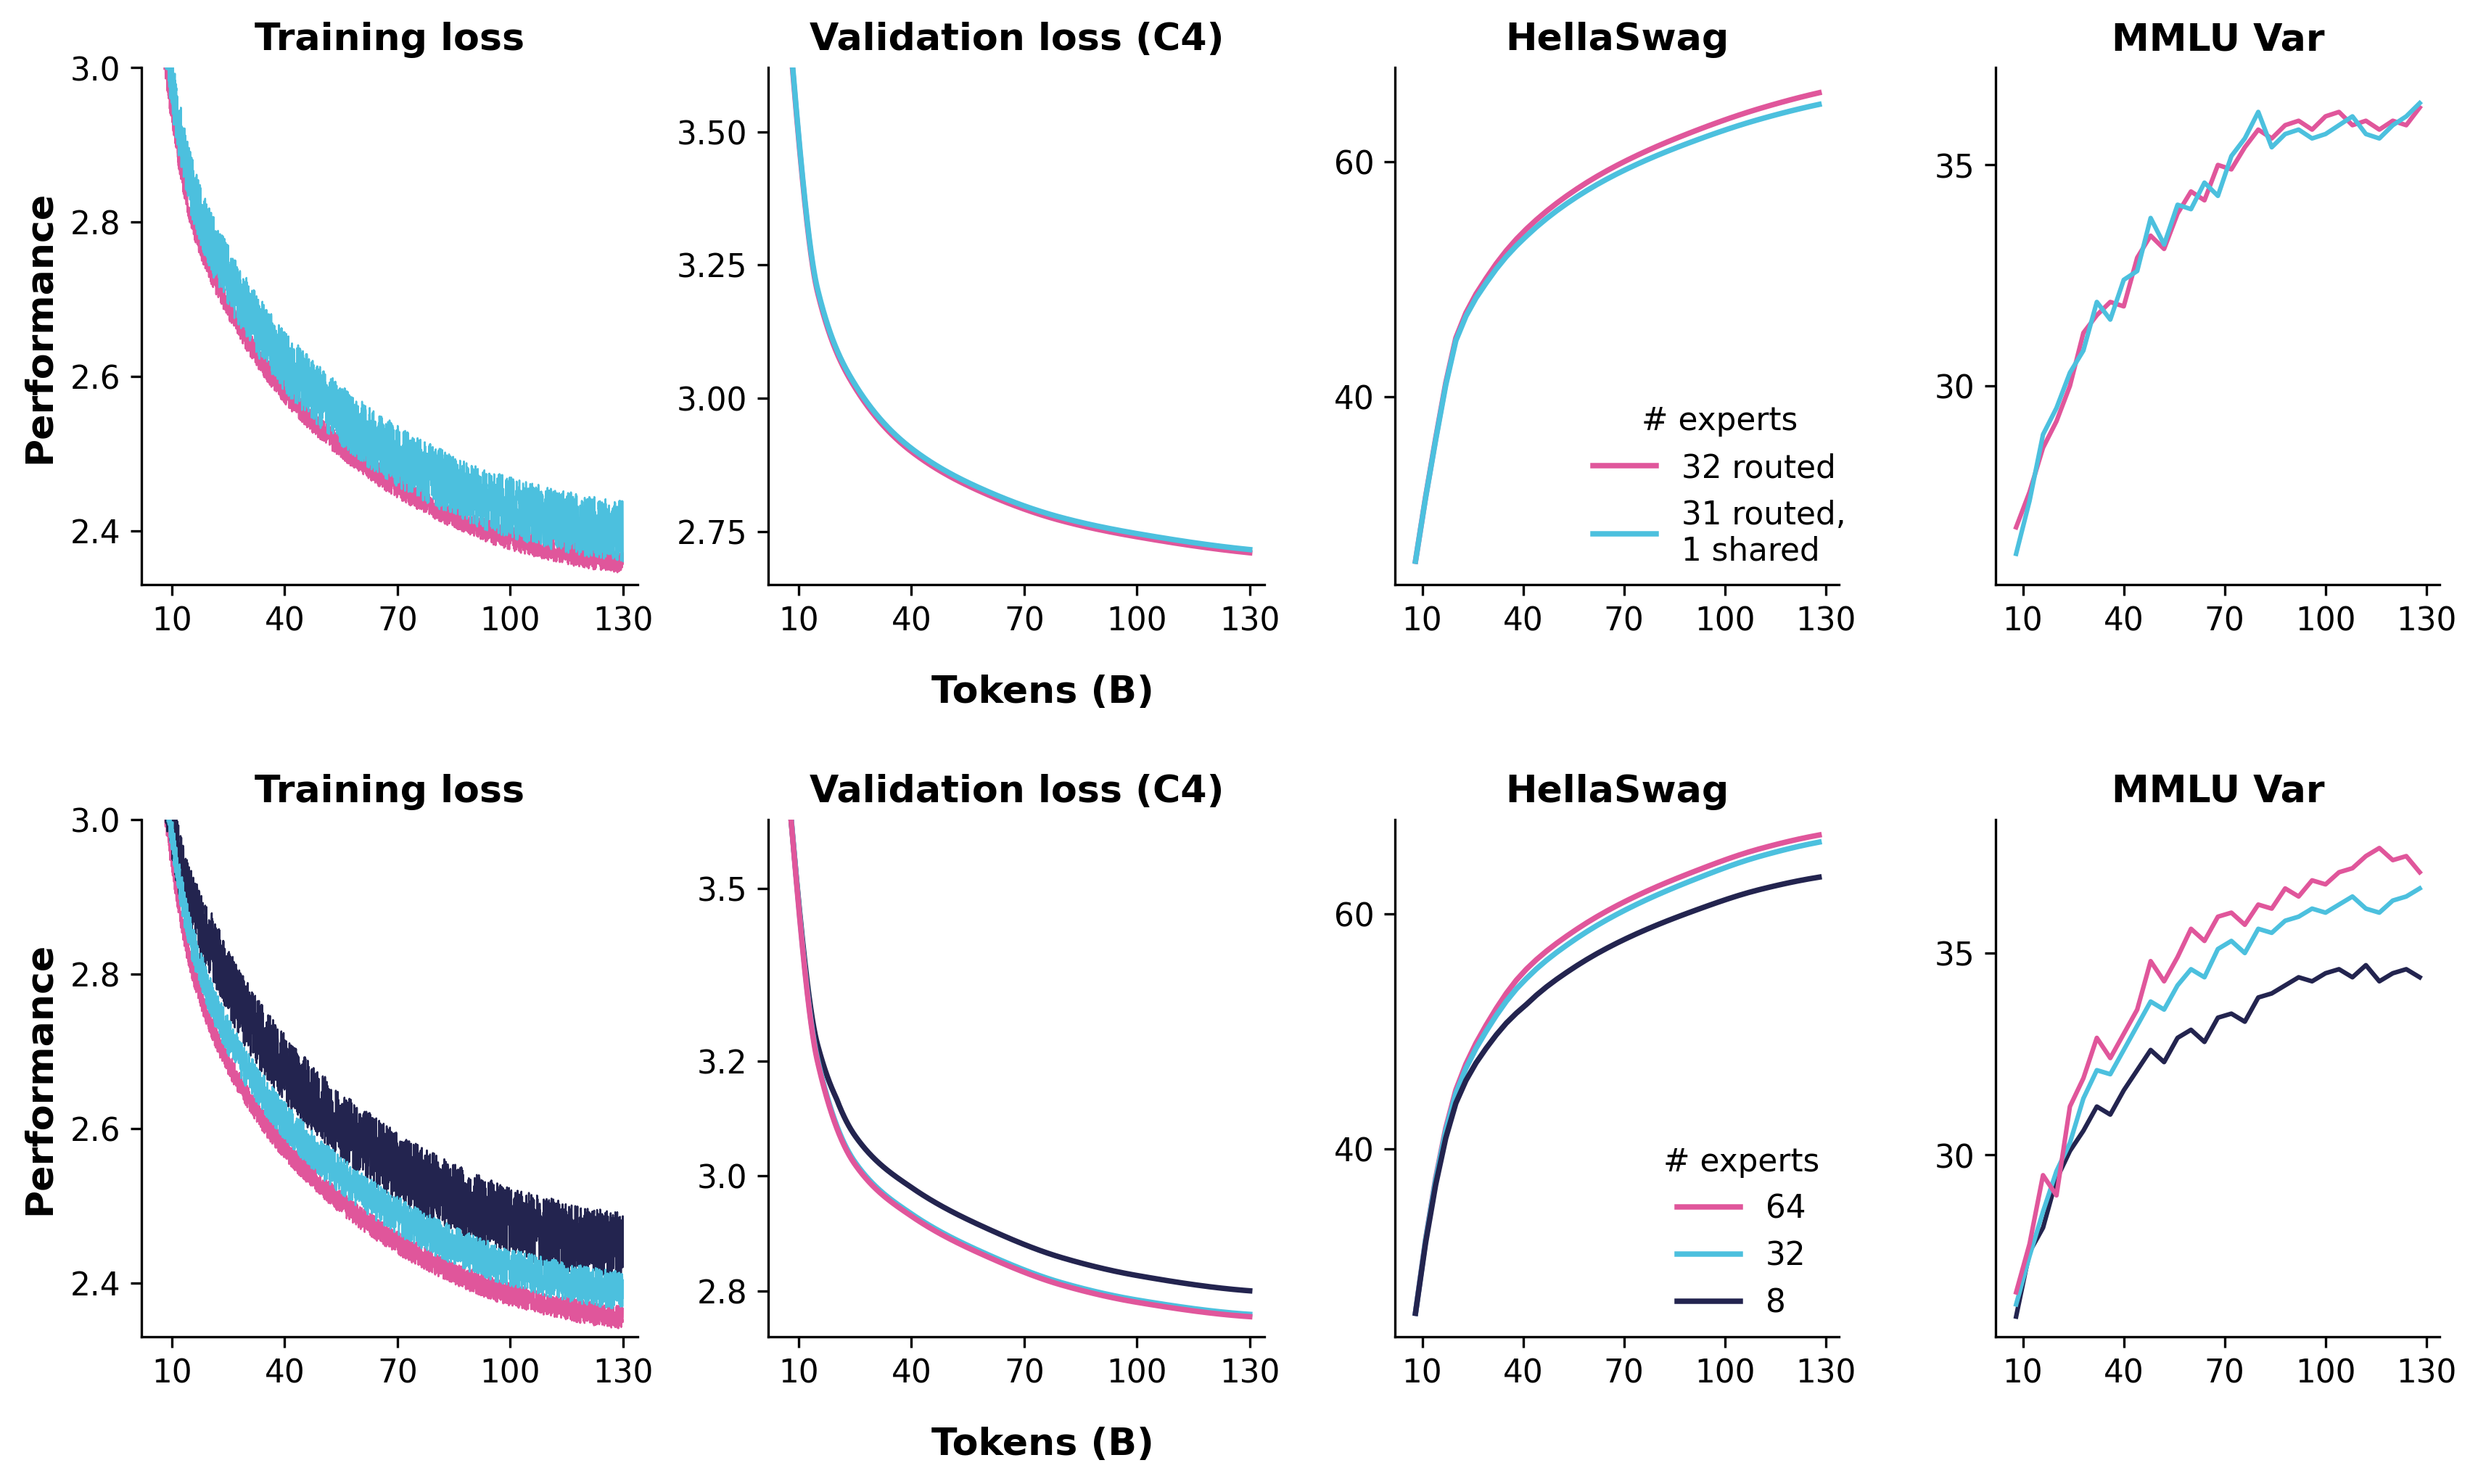
\includegraphics[width=1\linewidth]{olmoe.png}
\end{figure}

\subsection*{Expert routing setups for recent MoEs}

\begin{figure}[H]
    \centering
    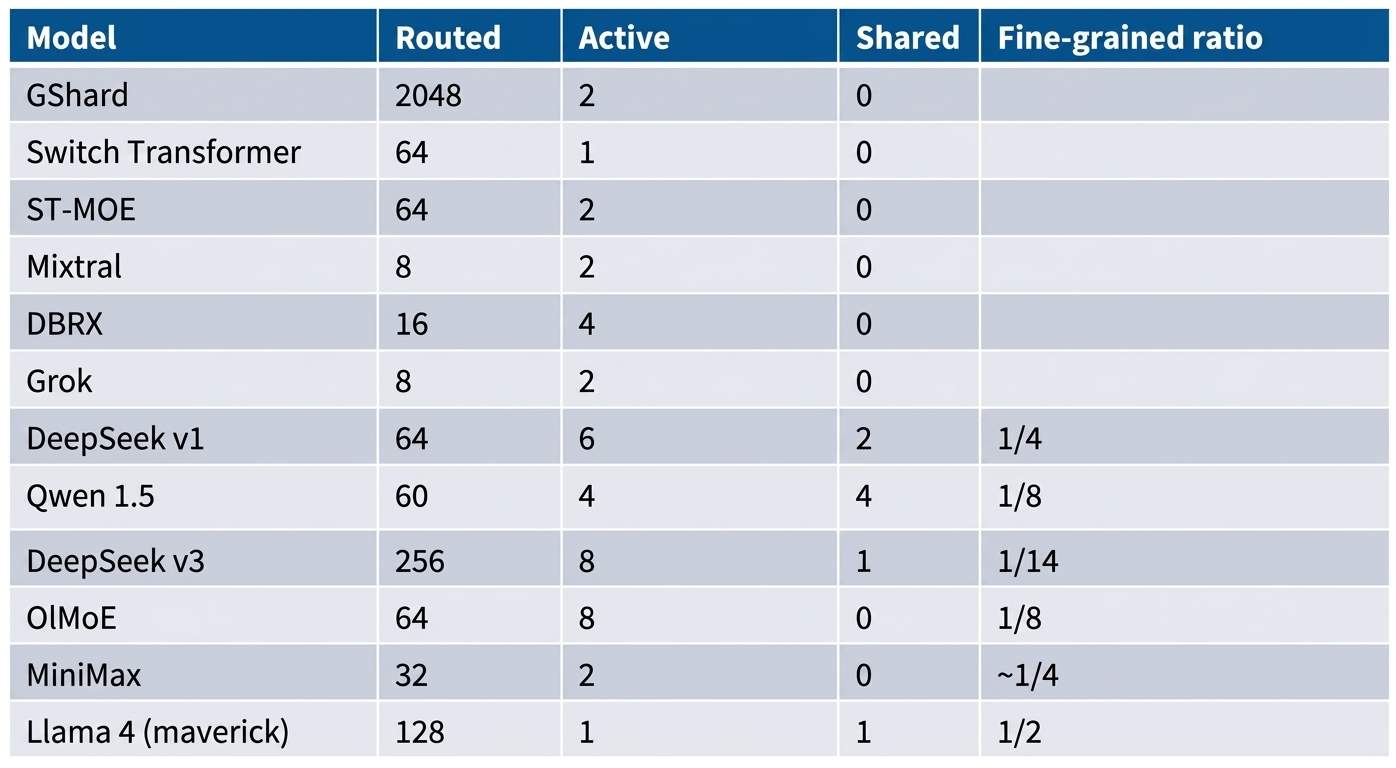
\includegraphics[width=1\linewidth]{chart.jpg}
\end{figure}

\subsection*{How to Train our MoEs?}

\begin{remark}
    We need sparsity for training-time efficiency ... but sparse gating decisions are not differentiable.\textbf{}
\end{remark}

\textbf{Solutions?}

\begin{enumerate}
    \item Reinforcement learning to optimize gating policies. 
    \item Stochastic perturbations.
    \item Heuristic "balancing" losses. 
\end{enumerate}

Guess which one people use in practice?

\subsubsection*{RL for MoEs}

\begin{itemize}
    \item RL via REINFORCEMENT does work, but not so much better that it's a clear win. 
    \item RL is the "right solution" but gradient variances and complexities means it's not widely used.
\end{itemize}

\subsubsection*{Stochastic approximations}

\begin{figure}[H]
    \centering
    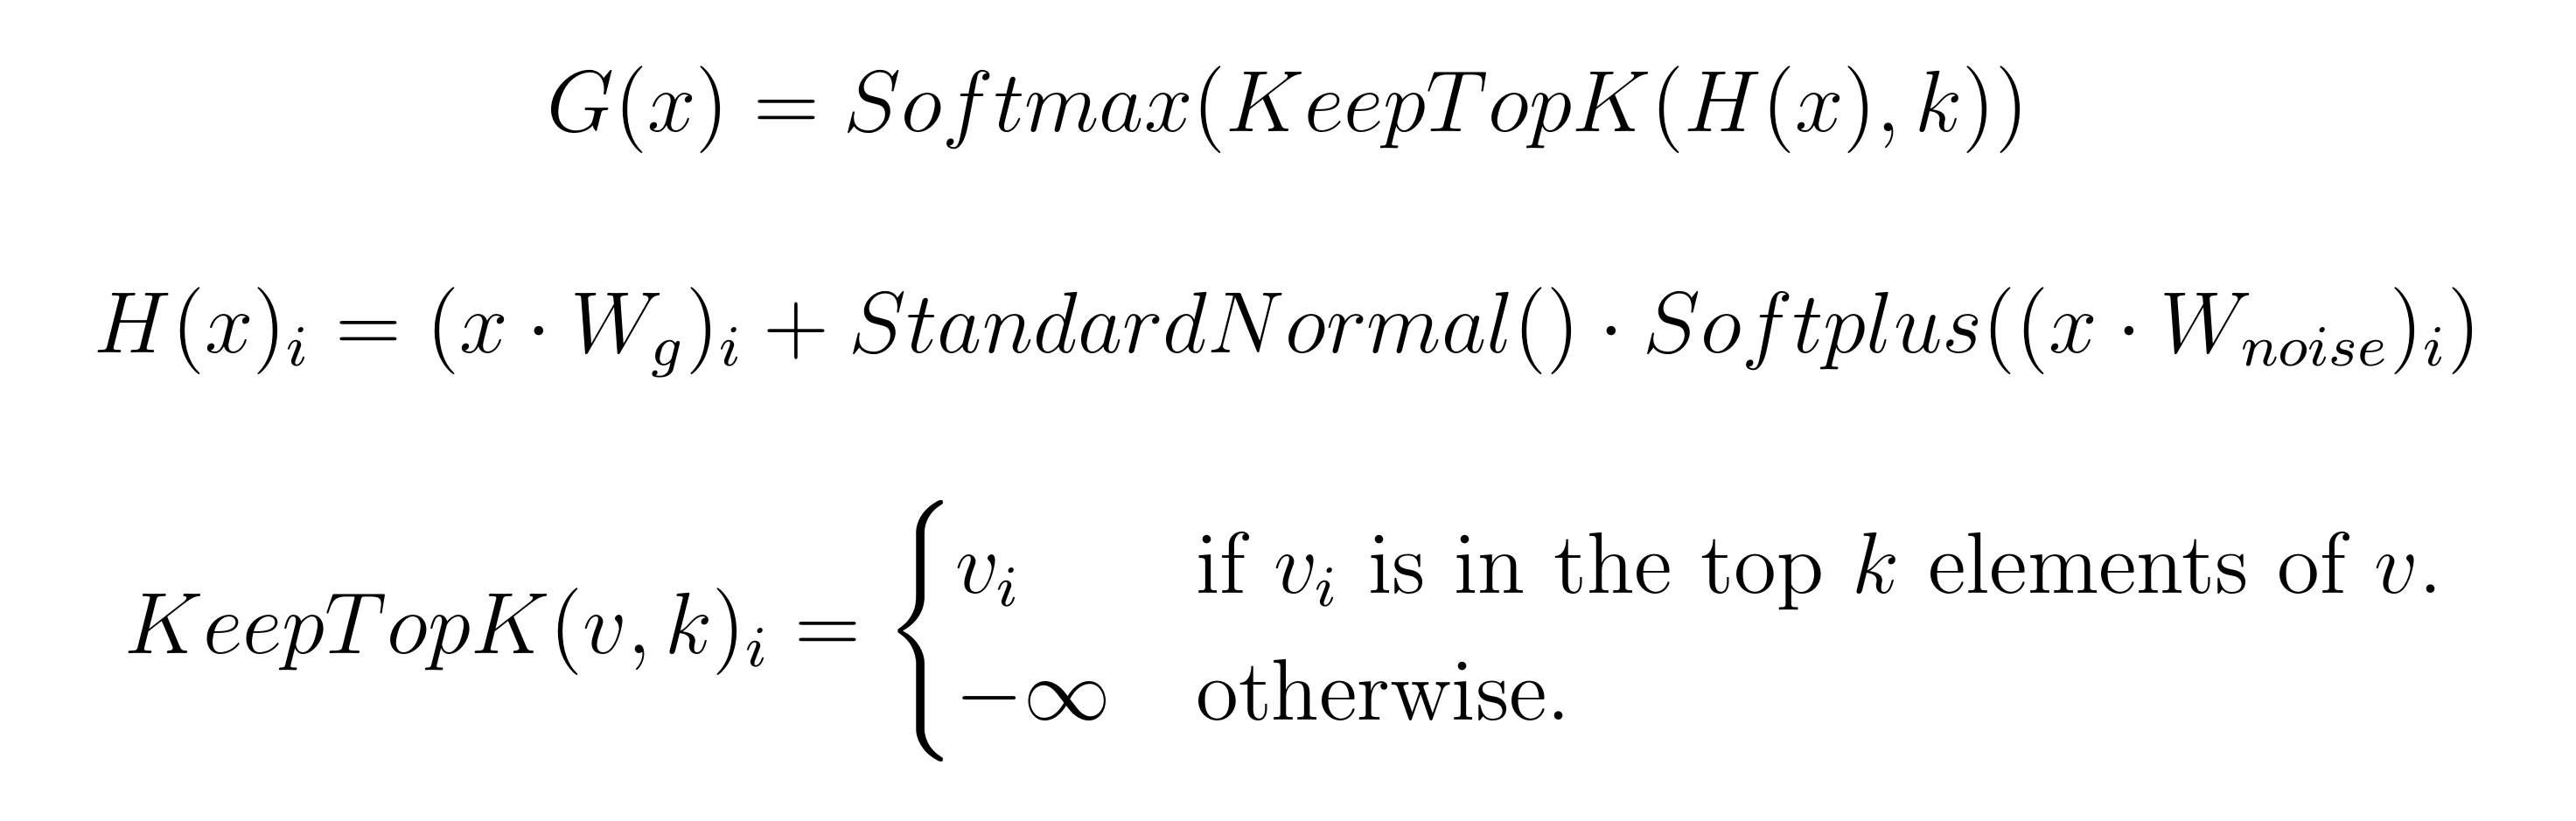
\includegraphics[width=1\linewidth]{SA.png}
\end{figure}

From Shazeer et al 2017 - routing decisions are \textit{stochastic} with Gaussian perturbations.
\begin{enumerate}
    \item This naturally leads to experts that are a bit more robust.
    \item The softmax means that the model learns how to rank \(k\) experts.
\end{enumerate}

\subsubsection*{Stochastic jitters}

\begin{minted}{python}
    if is_training:
        # Add noise for exploration across experts.
        router_logits += mtf.random_unform(
            shape=router_logits.shape, minval=1-eps, maxval=1+eps)
    
    # Convert input to softmax from bf16 to fp32 for stability.
    router_logits = mtf.to_float32(router_logits)
    
    # Probabilitites for each token.
    router_probs = mtf.softmax(router_logits, axis=-1)
\end{minted}

Stochastic jitter in Fedus et al 2022. This does uniform multiplicative perturbations for the same goal of getting less brittle experts. This was later removed in Zoph et al 2022.

\subsubsection*{Heuristic balancing losses}

Another key issue - systems efficiency requires that we use experts evenly ... \\

For each Switch layer, this auxiliary loss is added to the total model loss during training. Given \(N\) experts indexed by \(i = 1\) to \(N\) and a batch \(\mathcal{B}\) with \(T\) tokens, the auxiliary loss is computed as the scaled dot-product between vectors \(f\) and \(P\),
\[
    \operatorname{loss} = \alpha \cdot N \cdot \sum_{i = 1}^{N}f_i \cdot P_i
\]
where \(f_i\) is the fraction of tokens dispatched to expert \(i\),
\[
    f_i = \frac{1}{T}\sum_{x \in \mathcal{B}}\mathbf{1}\{\operatorname{argmax} p(x) = i\}
\]
and \(P_i\) is the fraction of the router probability allocated for expert \(i\),
\[
  P_i = \frac{1}{T}\sum_{x \in \mathcal{B}}p_i(x).  
\]

The derivative with respect to \(p_i(x)\) is 
\[
    \frac{\alpha N}{T^2}\sum_{}\mathbf{1}\{\operatorname{argmax} p(x) = i\},
\]
so more frequent use \(=\) stronger downweighting.

\subsubsection*{Example from DeepSeek (v1-2)}

\textbf{Per-expert balancing} - same as the above heuristic.
\begin{align*}
    \mathcal{L}_{\text{ExpBal}} &= \alpha_1 \sum_{i = 1}^{N'}f_iP_i, \\
    f_i &= \frac{N'}{K'T}\sum_{t = 1}^{T}\mathbf{1}(\text{Token } t \text{ selects Expert } i), \\
    P_i &= \frac{1}{T}\sum_{t = 1}^T s_i,t.
\end{align*}

\textbf{Per-device balancing} - the objective above, but aggregated by device.
\begin{align*}
    \mathcal{L}_{\text{DevBal}} &= \alpha_2\sum_{i = 1}^{D}f_i'P_i', \\
    f_i' &= \frac{1}{\vert \epsilon_i \vert}\sum_{j \in \epsilon_i}f_j, \\
    P_i' &= \sum_{j \in \epsilon_i}P_j.
\end{align*}

\subsubsection*{DeepSeek v3 variation - perExpert biases}

Set up a per-expert bias (making it more likely to get tokens) and use online learning.

\begin{figure}[H]
    \centering
    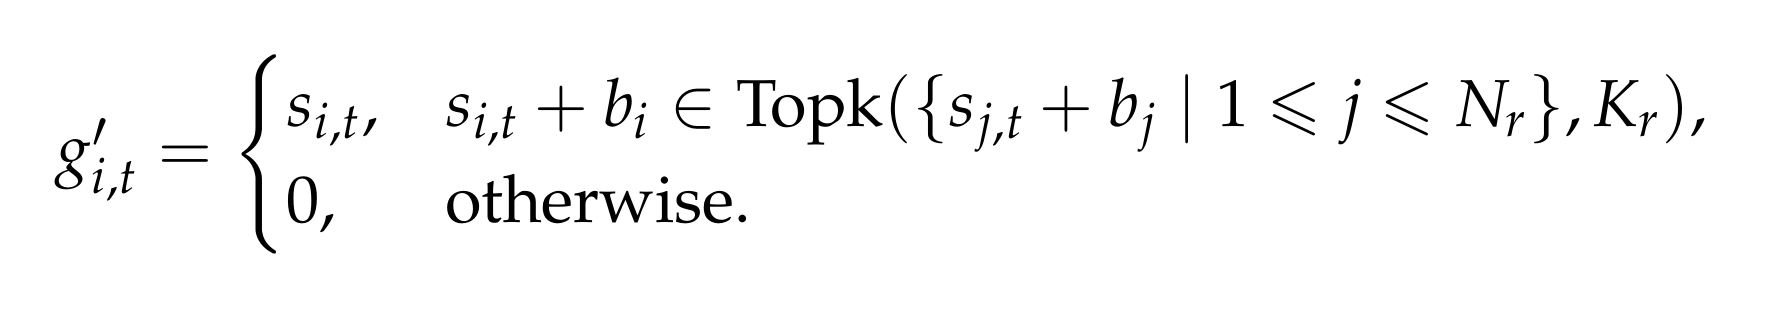
\includegraphics[width=1\linewidth]{variation.png}
\end{figure}

They call this "\textbf{auxiliary loss free balancing}" (but the approach is not fully auxiliary loss free ..) \\

\begin{center}
    Although DeepSeek-v3 mainly relies on the auxiliary-loss strategy for load balance, to prevent extreme imbalance within any single sequence, we also employ a complementary sequence-wise balance loss:
\end{center}
\begin{align*}
    \mathcal{L}_{\text{Bal}} &= \alpha \sum_{i = 1}^{N_r}f_i P_i, \\
    f_i &= \frac{N_r}{K_rT}\sum_{t = 1}^{T} \mathbf{1}(s_{i,t} \in \text{Topk}(\{s_{j,t} \mid 1 \leq j \neq N_r\}, K_r)), \\
    s'_{i,t} &= \frac{s_{i,t}}{\sum_{j = 1}^{N_r}s_{j,t}}, \\
    P_i &= \frac{1}{T} \sum_{t = 1}^{T} s'_{i,t}.
\end{align*}

\subsubsection*{Training MoEs - the systems side}

MoEs parallelize nicely - each FFN can fit in a device AND enable additional kinds of parallelism.

\begin{figure}[hpbt]
    \centering
    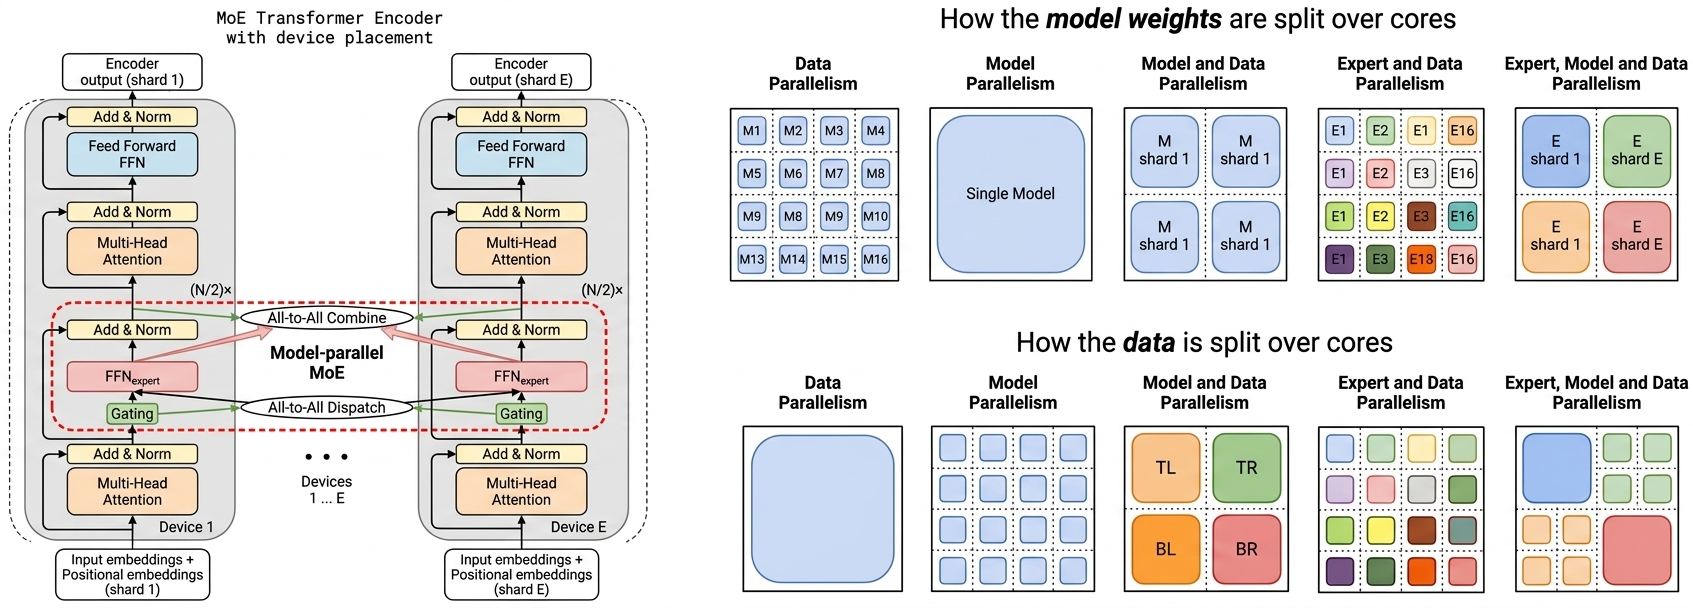
\includegraphics[width=1\linewidth]{devices.jpg}
\end{figure}

MoE routing allows for parallelism, but also some complexities.

\begin{figure}[hpbt]
    \centering
    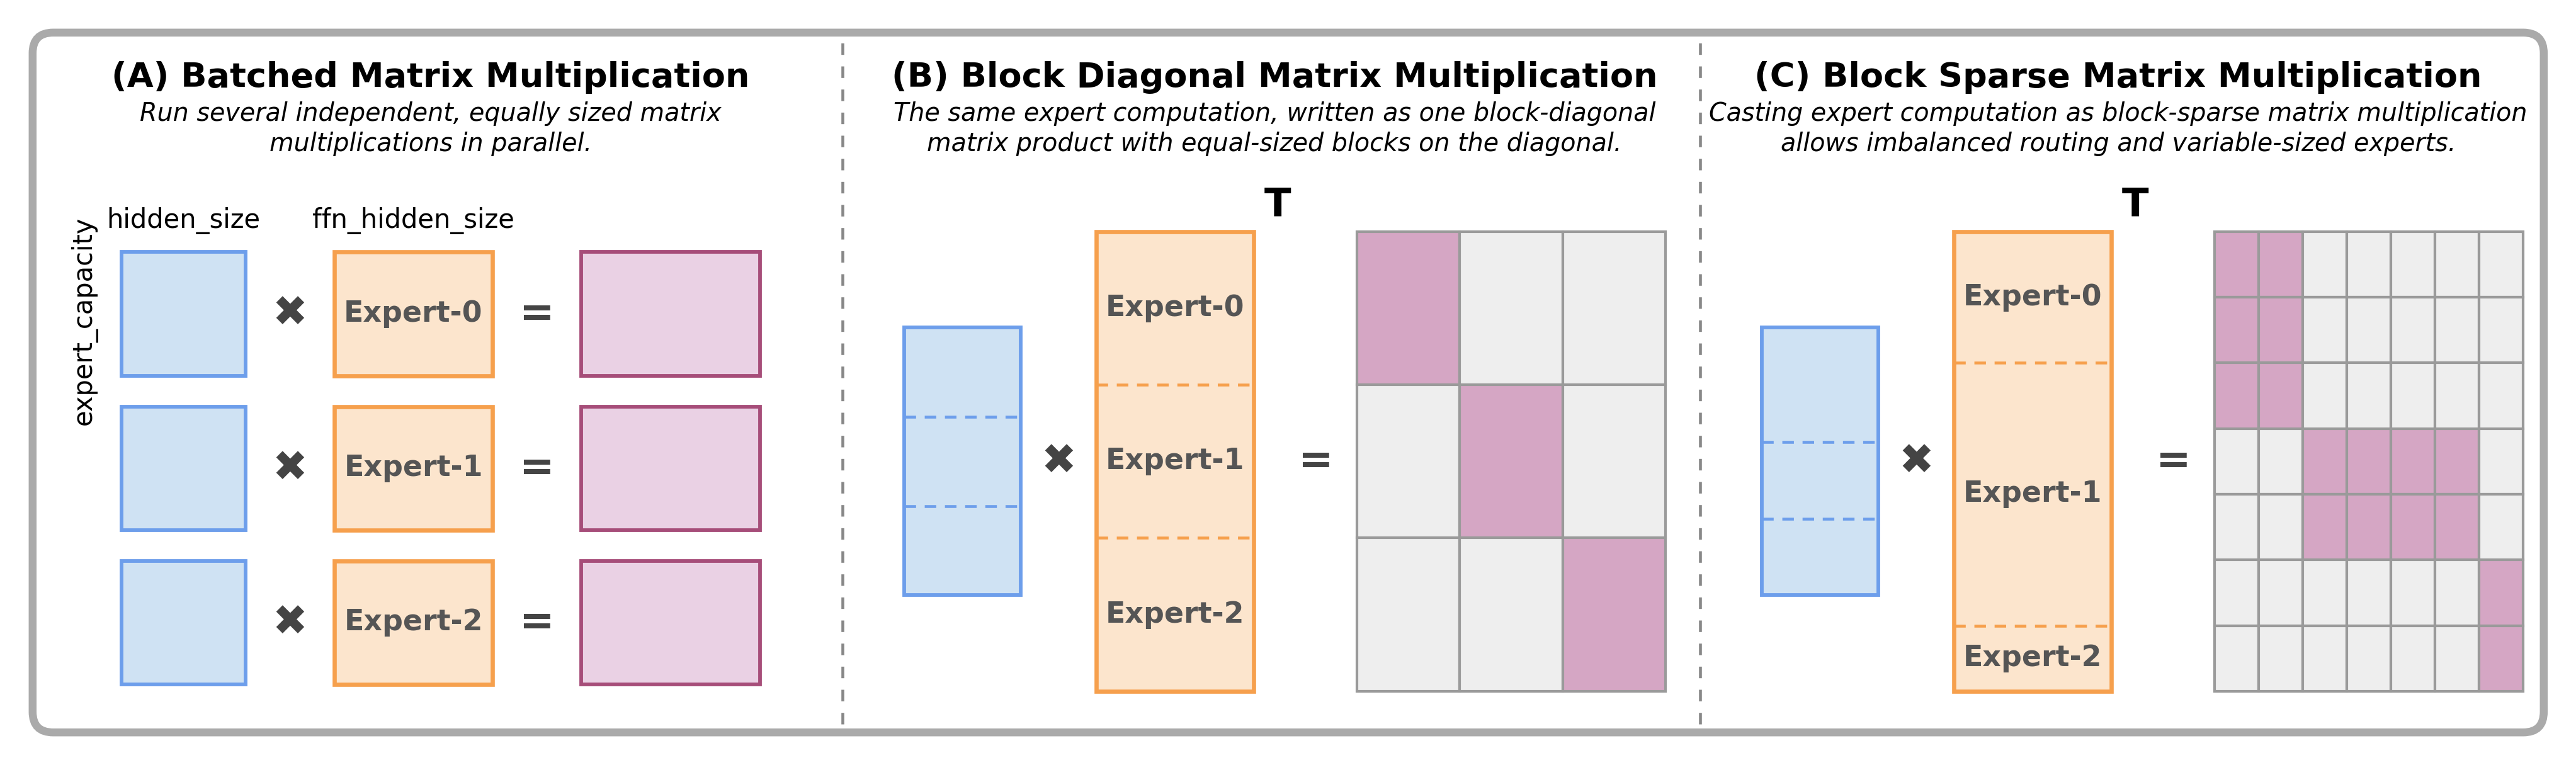
\includegraphics[width=1\linewidth]{matrices.png}
\end{figure}

Modern libraries like MegaBlocks (used in many open MoEs) use smarter sparse MatMuls.

\subsubsection*{Fun side issue - stochasticity of MoE models}

MoEs can have additional stochasticity beyond normal models ...

\begin{question}
    Why would a MoE have additional randomness?
\end{question}

\begin{figure}[hpbt]
    \centering
    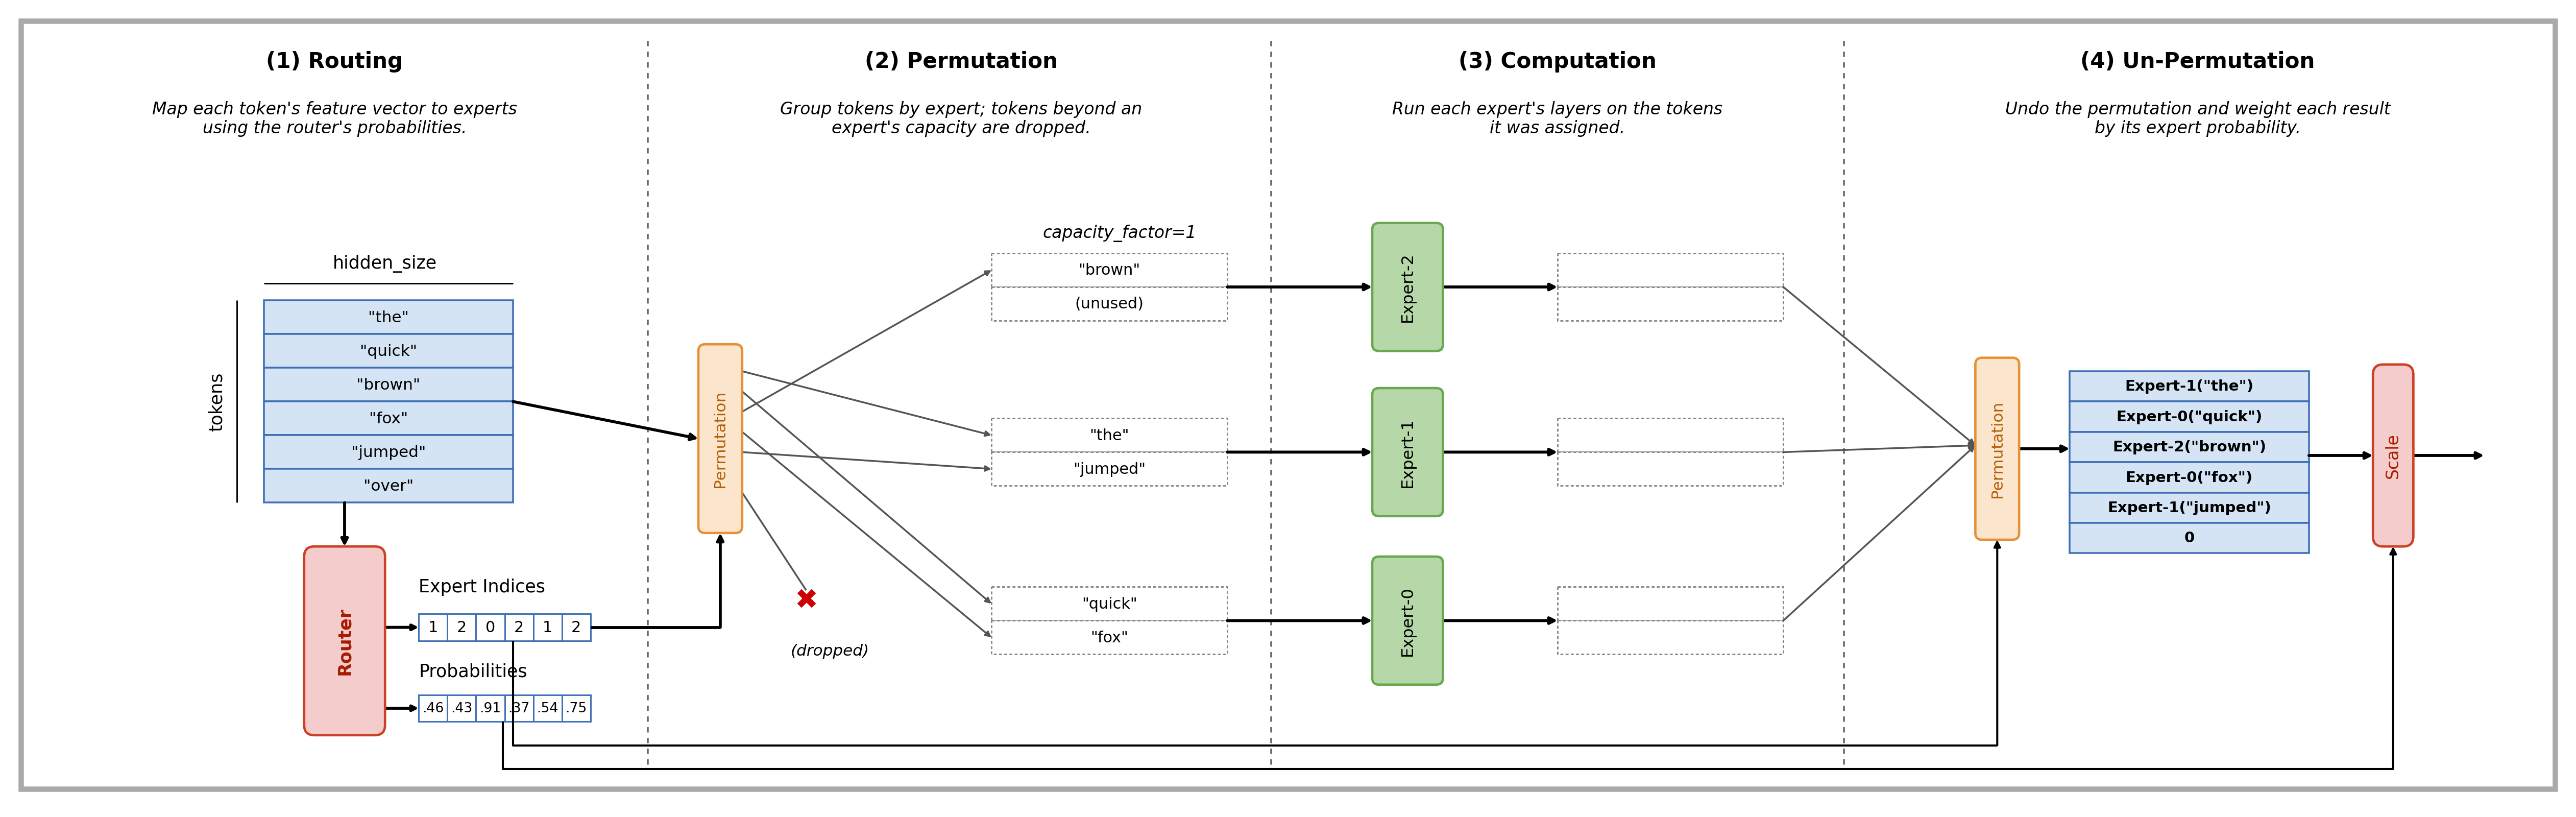
\includegraphics[width=1\linewidth]{random.png}
\end{figure}

Token dropping from routing happens at a \textit{batch} level - this means that other people's queries can drop your token.

\subsubsection*{Issues with MoEs - fineTuning}

\begin{itemize}
    \item Sparse MoEs can overfit on smaller fine-tuning data.
    \item Zoph et al solution - finetune nonMoE MLPs.
    \item DeepSeek solution - use lots of data (1.4M SFT).
\end{itemize}

\subsubsection*{Other training methods - upcycling}

\begin{question}
    Can we use a pretrained LM to initialize an MoE?
\end{question}

\begin{enumerate}[label=(\alph*)]
    \item Use the MiniCPM model (top\(k = 2\), 8 experts, 4B active parameters).
    \item Simple MoE, shows gains from the base model with 520B tokens for training.
    \item Initialize from the Qwen 1.8B model (top\(k = 4\), 60 experts with 4 shared).
    \item Similar architecture to DeepSeek MoE, but one of the first (confirmed) upcycling successes. 
\end{enumerate}

\subsubsection*{DeepSeek MoE v1-v2-v3}

To wrap up, we'll walk through the DeepSeek MoE architrcture.

\begin{enumerate}[label=(\Roman*)]
    \item \textbf{v1 (16B - 2.8 active):} Shared (2) \(+\) Fine-grained (64/4) experts \(/\) Standard, top-\(k\) routing \(/\) Standard Aux-loss balancing (Expert \(+\) Device).
    \item \textbf{v2 (236B - 21 active):} Shared (2) \(+\) Fine-grained (160/10) experts (6 active) \(/\) New, top-\(M\) device routing \(/\) Communication balancing loss - balancing both communication in \textit{and} out. 
    \item \textbf{v3 (671B - 37 active):} Shared (1) \(+\) Fine-grained (258) experts (8 active) \(/\) New Sigmoid \(+\) Softmax top-\(k\) + top-\(M\) \(/\) Aux-loss-free + seq-wise aux.
\end{enumerate}

\subsubsection*{Bonus: What else do you need to make DeepSeek MoE v3?}

\textbf{MLA:} multihead, latent attention! 

\begin{figure}[hpbt]
    \centering
    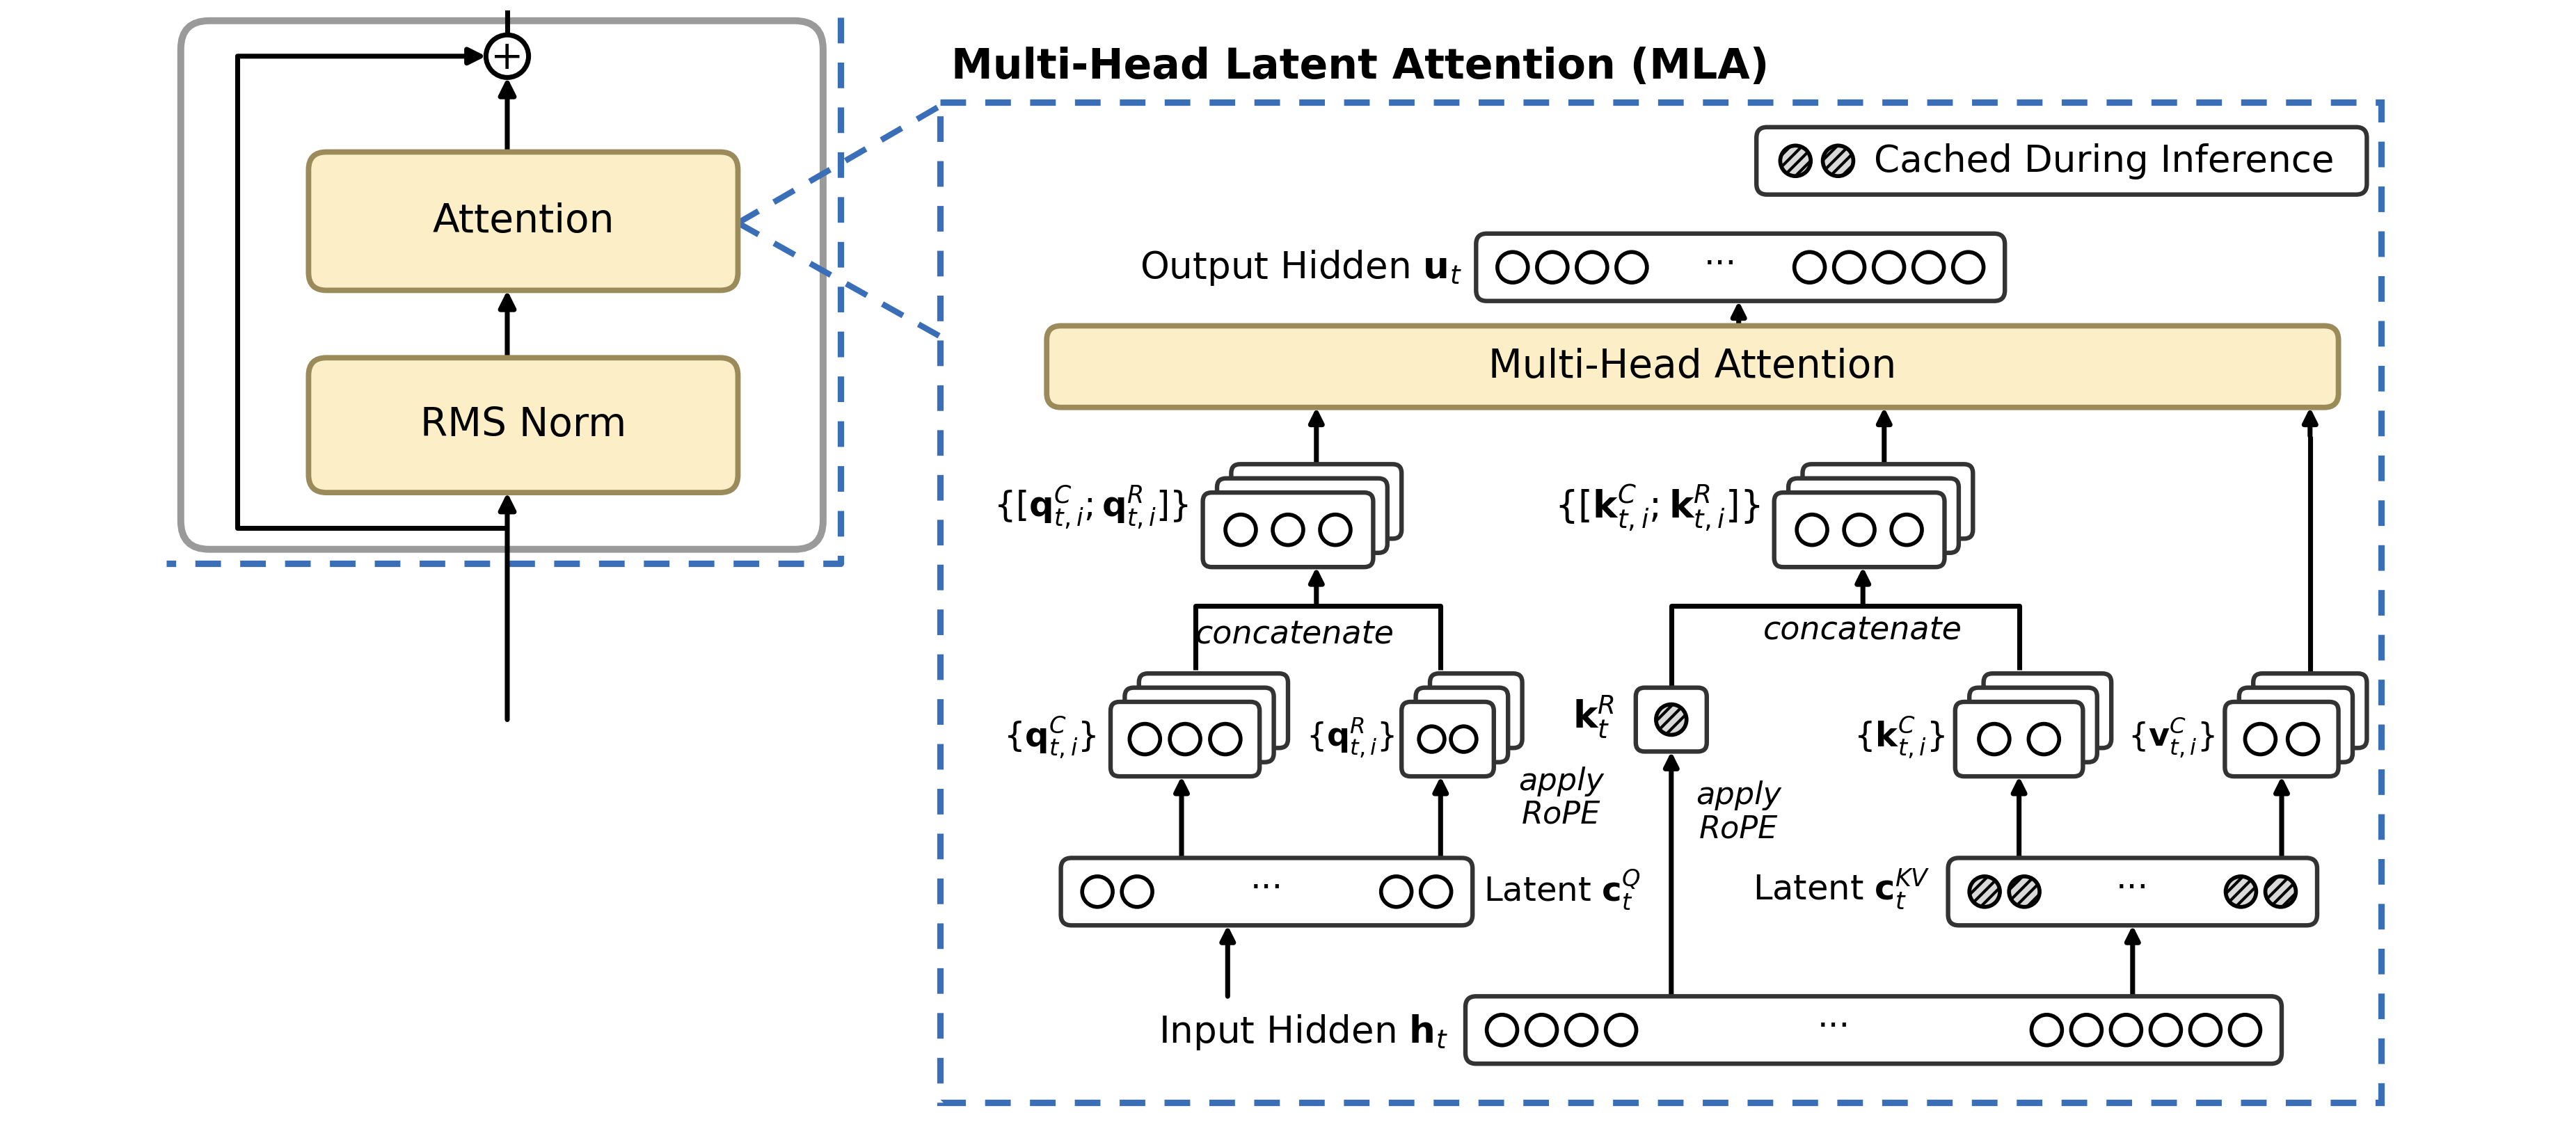
\includegraphics[width=1\linewidth]{mla.png}
\end{figure}

\begin{itemize}
    \item \textbf{Basic idea:} express the \(Q\), \(K\), \(V\) as functions of a lower dim, "latent" activation.
    \begin{align*}
        \mathbf{c}_t^{KV} &= W^{DKV} \mathbf{h}_t, \\
        \mathbf{k}_t^C &= W^{UK} \mathbf{c}_t^{KV}, \\
        \mathbf{v}_t^{C} &= W^{UK} \mathbf{c}_t^{KV}.
    \end{align*}
    \item \textbf{Benefits:} when \(KV\) caching, we only need to store \(\mathbf{c}_t^{KV}\), which can be much smaller (they also compress queries, for memory savings during training). 
    \begin{align*}
        \mathbf{c}_t^{Q} &= W^{DQ} \mathbf{h}_t, \\
        \mathbf{q}_t^C &= W^{UQ} \mathbf{c}_t^{Q}.
    \end{align*}
    \item \textbf{Complexity:} RoPE conflicts with MLA-style caching (the solution - have a few non-latent key dimensions that can be rotated).
    \begin{align*}
        &\text{Without RoPE - } \langle Q, K \rangle = \langle hW^Q, W^{UK}\mathbf{c}_t^{KV} \rangle = \langle hW^QW^{UK}, \mathbf{c}_t^{KV} \rangle \\
        &\text{With RoPE - } \langle QR_q, R_kK \rangle = \langle hW^QR_q, R_kW^{UK}\mathbf{c}_t^{KV} \rangle = \langle hW^QR_qR_kW^{UK}, \mathbf{c}_t^{KV} \rangle 
    \end{align*}
\end{itemize}

\textbf{MTP:} have small, lightweight models that predict multiple steps ahead.

\begin{figure}[H]
    \centering
    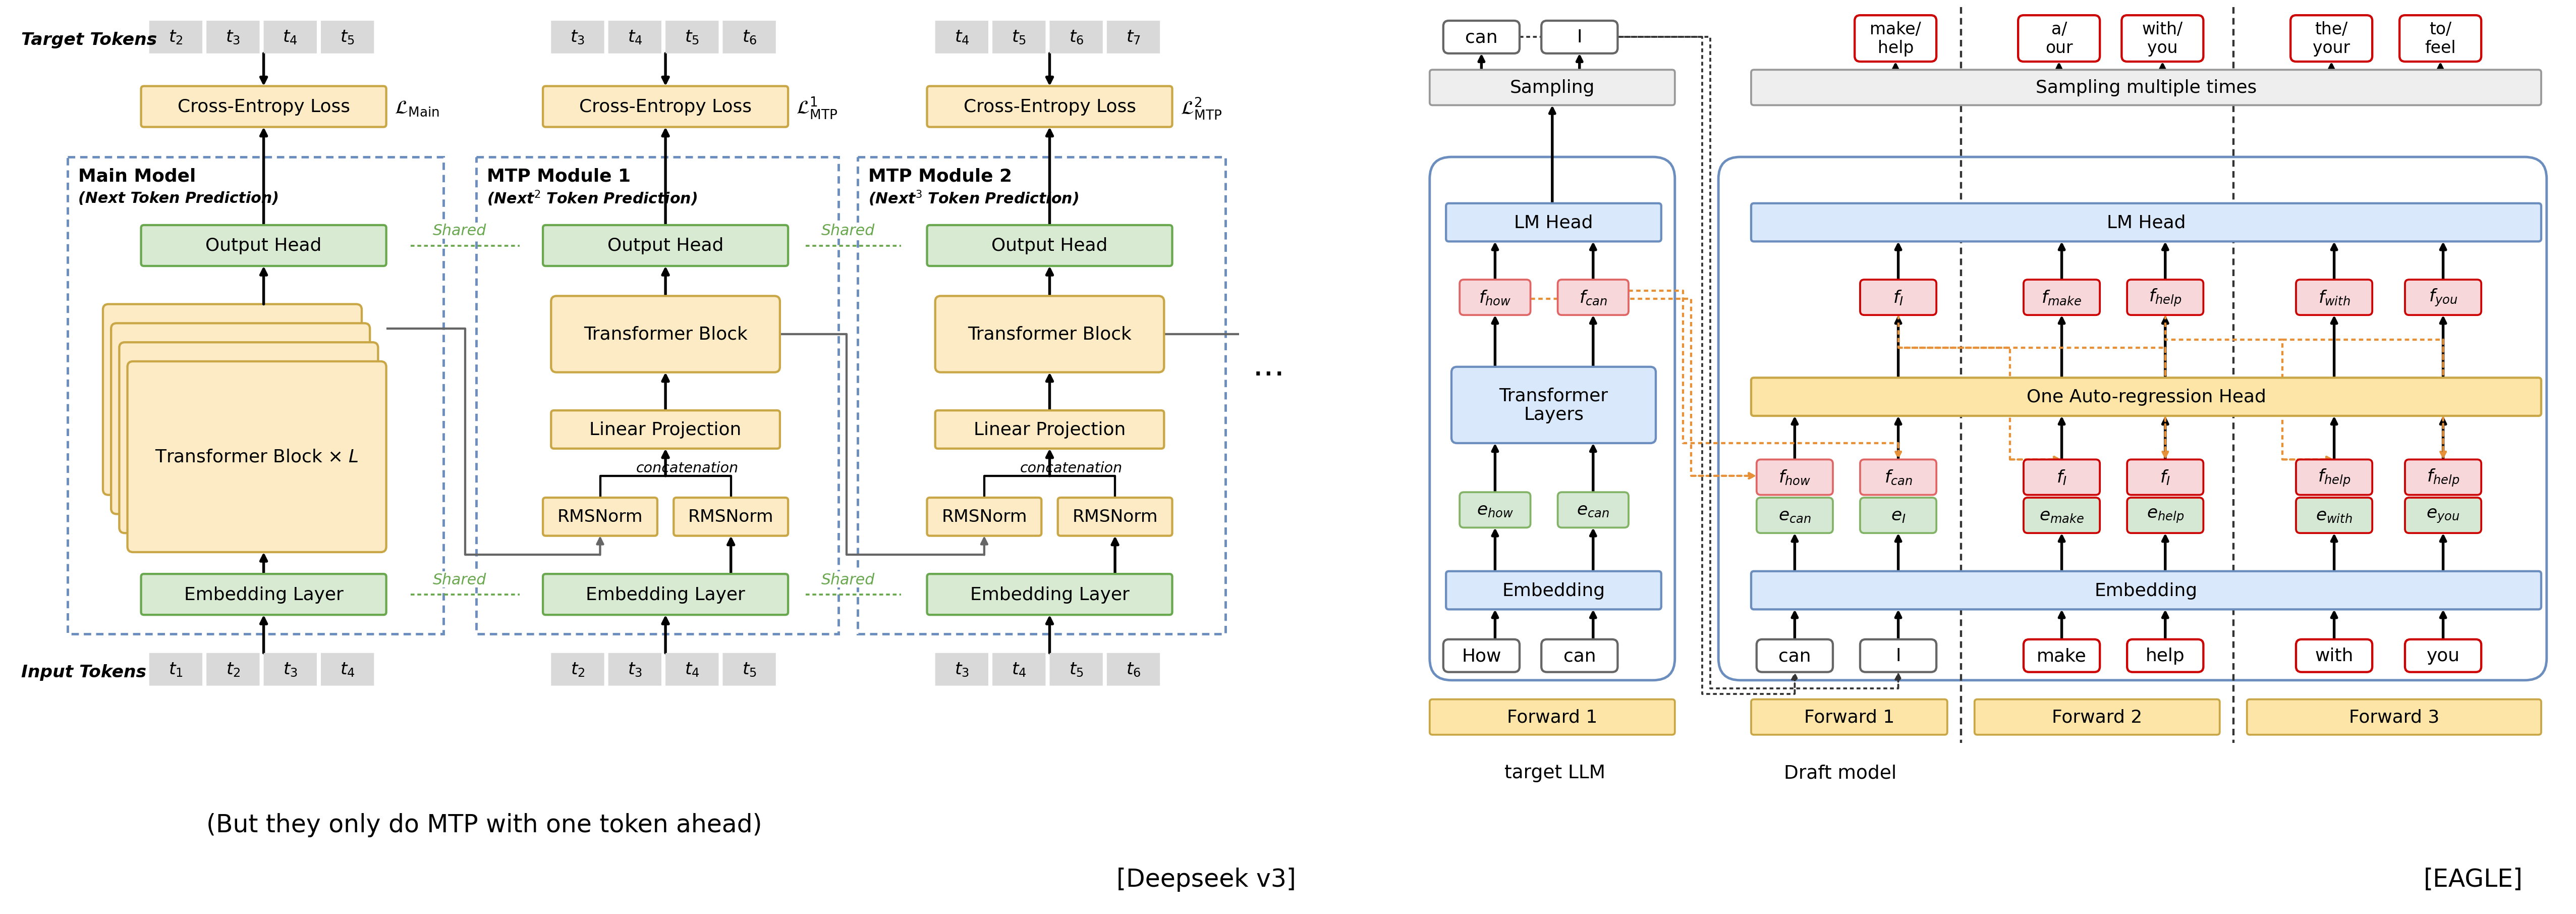
\includegraphics[width=1\linewidth]{mtp.png}
\end{figure}

\end{document}
